\PassOptionsToPackage{unicode=true}{hyperref} % options for packages loaded elsewhere
\PassOptionsToPackage{hyphens}{url}
%
\documentclass[]{article}
\usepackage{lmodern}
\usepackage{amssymb,amsmath}
\usepackage{ifxetex,ifluatex}
\usepackage{fixltx2e} % provides \textsubscript
\ifnum 0\ifxetex 1\fi\ifluatex 1\fi=0 % if pdftex
  \usepackage[T1]{fontenc}
  \usepackage[utf8]{inputenc}
  \usepackage{textcomp} % provides euro and other symbols
\else % if luatex or xelatex
  \usepackage{unicode-math}
  \defaultfontfeatures{Ligatures=TeX,Scale=MatchLowercase}
\fi
% use upquote if available, for straight quotes in verbatim environments
\IfFileExists{upquote.sty}{\usepackage{upquote}}{}
% use microtype if available
\IfFileExists{microtype.sty}{%
\usepackage[]{microtype}
\UseMicrotypeSet[protrusion]{basicmath} % disable protrusion for tt fonts
}{}
\IfFileExists{parskip.sty}{%
\usepackage{parskip}
}{% else
\setlength{\parindent}{0pt}
\setlength{\parskip}{6pt plus 2pt minus 1pt}
}
\usepackage{hyperref}
\hypersetup{
            pdftitle={The Woods Hole Assessment Model (WHAM): Incorporating environmental covariates into a state-space assessment framework},
            pdfauthor={Brian C. Stock1, Timothy J. Miller 1},
            pdfborder={0 0 0},
            breaklinks=true}
\urlstyle{same}  % don't use monospace font for urls
\usepackage[margin=1in]{geometry}
\usepackage{graphicx,grffile}
\makeatletter
\def\maxwidth{\ifdim\Gin@nat@width>\linewidth\linewidth\else\Gin@nat@width\fi}
\def\maxheight{\ifdim\Gin@nat@height>\textheight\textheight\else\Gin@nat@height\fi}
\makeatother
% Scale images if necessary, so that they will not overflow the page
% margins by default, and it is still possible to overwrite the defaults
% using explicit options in \includegraphics[width, height, ...]{}
\setkeys{Gin}{width=\maxwidth,height=\maxheight,keepaspectratio}
\setlength{\emergencystretch}{3em}  % prevent overfull lines
\providecommand{\tightlist}{%
  \setlength{\itemsep}{0pt}\setlength{\parskip}{0pt}}
\setcounter{secnumdepth}{5}
% Redefines (sub)paragraphs to behave more like sections
\ifx\paragraph\undefined\else
\let\oldparagraph\paragraph
\renewcommand{\paragraph}[1]{\oldparagraph{#1}\mbox{}}
\fi
\ifx\subparagraph\undefined\else
\let\oldsubparagraph\subparagraph
\renewcommand{\subparagraph}[1]{\oldsubparagraph{#1}\mbox{}}
\fi

% set default figure placement to htbp
\makeatletter
\def\fps@figure{htbp}
\makeatother

\usepackage{url}
\usepackage{setspace}
%\singlespacing
%\onehalfspacing
\doublespacing
\usepackage{lineno}
\linenumbers
\usepackage[belowskip=0pt,aboveskip=0pt]{caption}
\usepackage{booktabs}
\usepackage{longtable}
\usepackage{array}
\usepackage{multirow}
\usepackage{wrapfig}
\usepackage{float}
\usepackage{colortbl}
\usepackage{pdflscape}
\usepackage{tabu}
\usepackage{threeparttable}
\usepackage{threeparttablex}
\usepackage[normalem]{ulem}
\usepackage{makecell}
\usepackage{xcolor}

\title{The Woods Hole Assessment Model (WHAM): Incorporating environmental
covariates into a state-space assessment framework}
\author{Brian C. Stock\textsuperscript{1}, Timothy J. Miller \textsuperscript{1}}
\date{}

\begin{document}
\maketitle

\(^1\)\href{mailto:brian.stock@noaa.gov}{\nolinkurl{brian.stock@noaa.gov}},
\href{mailto:timothy.j.miller@noaa.gov}{\nolinkurl{timothy.j.miller@noaa.gov}},
Northeast Fisheries Science Center, National Marine Fisheries Service,
166 Water Street, Woods Hole, MA 02543, USA\\

\pagebreak

\hypertarget{abstract}{%
\subsection*{Abstract}\label{abstract}}
\addcontentsline{toc}{subsection}{Abstract}

WHAM is great.

\hypertarget{keywords}{%
\subsubsection*{Keywords}\label{keywords}}
\addcontentsline{toc}{subsubsection}{Keywords}

state-space; stock assessment; mixed effects; random effects;
time-varying; Template Model Builder (TMB)

\pagebreak

\hypertarget{introduction}{%
\section{Introduction}\label{introduction}}

Grab stuff from NRC and Fish/Climate proposals.

\hypertarget{context-assessments-in-the-u.s.-northeast}{%
\subsection{Context: assessments in the U.S.
Northeast}\label{context-assessments-in-the-u.s.-northeast}}

\begin{itemize}
\tightlist
\item
  Long history, high F (pre-data)
\item
  Empirical weight-at-age
\item
  Retrospective patterns
\item
  ASAP3/4
\item
  Operational vs.~research-track
\item
  The Northeast U.S. Shelf LME is rapidly changing. Top priority is to
  ``continue development of stock assessment models that include
  environmental terms'' (Hare et al., 2016).
\end{itemize}

\hypertarget{motivation-1-advantages-of-state-space-stock-assessments}{%
\subsection{Motivation \#1: advantages of state-space stock
assessments}\label{motivation-1-advantages-of-state-space-stock-assessments}}

\begin{itemize}
\tightlist
\item
  objective estimation of process errors and data weighting, e.g.
  \(\sigma_R\), instead of ad-hoc
\item
  inherently predict unobserved states, so predicting missing data/years
  and into the future is natural
\item
  allow for time/age variation in demographic processes while estimating
  fewer parameters
\item
  natural framework to include environmental time-series
\item
  lower retros and AIC, larger (more realistic) uncertainty compared to
  SCAAs. Cite ICES state-space if in review.
\end{itemize}

(Aeberhard et al., 2018; Miller et al., 2016; Nielsen and Berg, 2014)

\hypertarget{motivation-2-allow-for-environmental-effects}{%
\subsection{Motivation \#2: allow for environmental
effects}\label{motivation-2-allow-for-environmental-effects}}

\begin{itemize}
\tightlist
\item
  Reduced retrospective patterns
\item
  Lower residual variance
\end{itemize}

(Miller et al., 2016; Miller and Hyun, 2018; O'Leary et al., 2019)

\hypertarget{how-is-wham-different-from-sam}{%
\subsection{How is WHAM different from
SAM?}\label{how-is-wham-different-from-sam}}

\emph{Not sure where to put this\ldots{} may be more natural after
introducing equations in Methods, some in Discussion. Definitely will be
a question in readers' minds so may be good to introduce early?}

Most assessments in the U.S. assume separability in \(F_{a,t}\),
estimate \(F_t\) and \(Sel_a\). WHAM does this. SAM estimates
\(F_{a,t}\) directly. WHAM and SAM also make different separability
assumptions for the catch/index data (aggregate total + age comps vs.
\(C_{a,t}\) directly). Should be similar (?) but could test.

Goal is to replicate ASAP assessments in the U.S. Northeast. Can easily
turn on/off random effects.

Observation model is natural for landings data that are measured as
total weight plus age composition sampling. Age composition sampling
often done separately with survey data.

Treating \(F\) and \(Sel\) separately can be useful for projections.
Oftentimes we want to specify \(F\) in projections to calculate a
reference point, as opposed to continuing a \(F\) time-series process.

\hypertarget{bias-correction}{%
\subsection{Bias correction}\label{bias-correction}}

\begin{itemize}
\tightlist
\item
  Analytical obs error. (Aldrin et al., 2020).
\item
  Analytical process error.
\item
  TMB epsilon. (Thorson, 2019; Thorson and Kristensen, 2016)
\end{itemize}

Should these all be used?

\hypertarget{overview}{%
\subsection{Overview}\label{overview}}

In summary, the NEFSC wants an assessment framework that i) estimates
random effects (i.e.~a state-space model), ii) includes environmental
effects, and iii) is easy to test against status quo SCAA models (ASAP).
The objectives of this manuscript are to introduce the WHAM framework
and demonstrate unbiasedness in self- and cross-tests.

\hypertarget{methods}{%
\section{Methods}\label{methods}}

\hypertarget{model-description}{%
\subsection{Model description}\label{model-description}}

\hypertarget{unobserved-states-random-effects}{%
\subsubsection{Unobserved states (random
effects)}\label{unobserved-states-random-effects}}

\hypertarget{numbers-at-age-survival}{%
\paragraph{Numbers-at-age (survival)}\label{numbers-at-age-survival}}

\hypertarget{natural-mortality-m}{%
\paragraph{\texorpdfstring{Natural mortality
(\(M\))}{Natural mortality (M)}}\label{natural-mortality-m}}

\hypertarget{selectivity}{%
\paragraph{Selectivity}\label{selectivity}}

\hypertarget{environmental-covariates}{%
\paragraph{Environmental covariate(s)}\label{environmental-covariates}}

\hypertarget{time-series-model}{%
\subparagraph{Time-series model}\label{time-series-model}}

\hypertarget{observation-model}{%
\subparagraph{Observation model}\label{observation-model}}

\hypertarget{link-to-population}{%
\subparagraph{Link to population}\label{link-to-population}}

\hypertarget{dataobservation-model}{%
\subsubsection{Data/observation model}\label{dataobservation-model}}

\hypertarget{catch-agg-age-comp}{%
\paragraph{Catch (agg, age comp)}\label{catch-agg-age-comp}}

\hypertarget{index-agg-age-comp}{%
\paragraph{Index (agg, age comp)}\label{index-agg-age-comp}}

\hypertarget{simulation-tests}{%
\subsection{Simulation tests}\label{simulation-tests}}

We used the stocks in Table \ref{tab:stock-list}.

We used R (R Core Team, 2020). WHAM is available as an R package (Miller
and Stock, 2020). OSA residuals.

\hypertarget{results}{%
\section{Results}\label{results}}

Sweet figures.

\hypertarget{discussion}{%
\section{Discussion}\label{discussion}}

\hypertarget{overview-1}{%
\subsection{Overview}\label{overview-1}}

We described WHAM. Sim tests showed no bias in self-tests (when
estimation model matched operating model). Some bias in cross-tests.

\hypertarget{future-work}{%
\subsection{Future work}\label{future-work}}

WHAM will be used in upcoming research track assessments. Could
transition to operational. Potential to improve several NEFSC
assessments.

\begin{itemize}
\tightlist
\item
  2D AR(1) selectivity. Most assessments in the U.S. assume separability
  in \(F_{a,t}\), i.e.~estimate \(F_t\) and \(Sel_a\). WHAM does this.
  SAM estimates \(F_{a,t}\) directly. WHAM and SAM make different
  separability assumptions for the catch/index data as well (aggregate
  total + age comps vs. \(C_{a,t}\) directly). Should be similar (?) but
  could test.
\item
  How many time/age-varying random effects can be estimated
  simultaneously? Stock et al. (n.d.) estimated random effect deviations
  in survival and \(M\), as well as an environmental covariate effect on
  recruitment.
\item
  Ecov-Recruitment simulation study. How much information does Ecov need
  to have to be useful?
\end{itemize}

\hypertarget{extensions}{%
\subsection{Extensions}\label{extensions}}

\hypertarget{multivariate-spatiotemporal-environmental-data}{%
\subsubsection{Multivariate spatiotemporal environmental
data}\label{multivariate-spatiotemporal-environmental-data}}

\hypertarget{lengthgrowth-estimation}{%
\subsubsection{Length/growth estimation}\label{lengthgrowth-estimation}}

\hypertarget{ecov-models}{%
\subsubsection{Ecov models}\label{ecov-models}}

\begin{itemize}
\tightlist
\item
  AR(k)
\item
  splines
\item
  Gaussian process/EDM/Munch/Sugihara
\end{itemize}

\hypertarget{conclusion}{%
\subsection{Conclusion}\label{conclusion}}

Development of TMB has facilitated significant advancement in fisheries
assessment, allowing us to treat population processes as random effects.
A grand challenge in fisheries is to assess and manage stocks in a
changing environment. Increasingly have the environmental data.
Population time-series are lengthening. WHAM is a step in this
direction.

\hypertarget{acknowledgements}{%
\subsection*{Acknowledgements}\label{acknowledgements}}
\addcontentsline{toc}{subsection}{Acknowledgements}

This research was performed while BCS held an NRC Research Associateship
award at the NEFSC. NOAA Fish \& Climate grant number.

\pagebreak

\hypertarget{supplementary-material}{%
\subsection*{Supplementary material}\label{supplementary-material}}
\addcontentsline{toc}{subsection}{Supplementary material}

More figures.

\pagebreak

\hypertarget{references}{%
\subsection*{References}\label{references}}
\addcontentsline{toc}{subsection}{References}

\hypertarget{refs}{}
\leavevmode\hypertarget{ref-aeberhard2018Review}{}%
Aeberhard, W.H., Mills Flemming, J., Nielsen, A., 2018. Review of
State-Space Models for Fisheries Science. Annu. Rev. Stat. Appl. 5,
215--235. \url{https://doi.org/10.1146/annurev-statistics-031017-100427}

\leavevmode\hypertarget{ref-aldrin2020Specification}{}%
Aldrin, M., Tvete, I., Aanes, S., Subbey, S., 2020. The specification of
the data model part in the SAM model matters. Fisheries Research 229,
105585. \url{https://doi.org/10.1016/j.fishres.2020.105585}

\leavevmode\hypertarget{ref-hare2016Northeast}{}%
Hare, J.A., Borggaard, D.L., Friedland, K.D., Anderson, J., Burns, P.,
Chu, K., Clay, P.M., Collins, M.J., Cooper, P., Fratantoni, P.S.,
Johnson, M.R., Manderson, J.P., Milke, L., Miller, T.J., Orphanides,
C.D., Saba, V.S., 2016. Northeast Regional Action Plan - NOAA Fisheries
Climate Science Strategy (No. NMFS-NE-239). NOAA Fisheries, Northeast
Fisheries Science Center, Woods Hole, MA.

\leavevmode\hypertarget{ref-miller2016Statespace}{}%
Miller, T.J., Hare, J.A., Alade, L.A., 2016. A state-space approach to
incorporating environmental effects on recruitment in an age-structured
assessment model with an application to southern New England yellowtail
flounder. Canadian Journal of Fisheries and Aquatic Sciences 73,
1261--1270. \url{https://doi.org/10.1139/cjfas-2015-0339}

\leavevmode\hypertarget{ref-miller2018Evaluating}{}%
Miller, T.J., Hyun, S.-Y., 2018. Evaluating evidence for alternative
natural mortality and process error assumptions using a state-space,
age-structured assessment model. Canadian Journal of Fisheries and
Aquatic Sciences 75, 691--703.
\url{https://doi.org/10.1139/cjfas-2017-0035}

\leavevmode\hypertarget{ref-miller2020Woods}{}%
Miller, T.J., Stock, B.C., 2020. The Woods Hole Assessment Model (WHAM).

\leavevmode\hypertarget{ref-nielsen2014Estimation}{}%
Nielsen, A., Berg, C.W., 2014. Estimation of time-varying selectivity in
stock assessments using state-space models. Fisheries Research 158,
96--101. \url{https://doi.org/10.1016/j.fishres.2014.01.014}

\leavevmode\hypertarget{ref-oleary2019Understanding}{}%
O'Leary, C.A., Miller, T.J., Thorson, J.T., Nye, J.A., 2019.
Understanding historical summer flounder ( \emph{Paralichthys}
\emph{Dentatus} ) abundance patterns through the incorporation of
oceanography-dependent vital rates in Bayesian hierarchical models. Can.
J. Fish. Aquat. Sci. 76, 1275--1294.
\url{https://doi.org/10.1139/cjfas-2018-0092}

\leavevmode\hypertarget{ref-rcoreteam2020Language}{}%
R Core Team, 2020. R: A Language and Environment for Statistical
Computing.

\leavevmode\hypertarget{ref-stockthisissueImplementing}{}%
Stock, B.C., Xu, H., Miller, T.J., Thorson, J.T., Nye, J.A., n.d.
Implementing a 2-dimensional smoother on either survival or natural
mortality improves a state-space assessment model for Southern New
England-Mid Atlantic yellowtail flounder.

\leavevmode\hypertarget{ref-thorson2019Perspective}{}%
Thorson, J.T., 2019. Perspective: Let's simplify stock assessment by
replacing tuning algorithms with statistics. Fisheries Research 217,
133--139. \url{https://doi.org/10.1016/j.fishres.2018.02.005}

\leavevmode\hypertarget{ref-thorson2016Implementing}{}%
Thorson, J.T., Kristensen, K., 2016. Implementing a generic method for
bias correction in statistical models using random effects, with spatial
and population dynamics examples. Fisheries Research 175, 66--74.
\url{https://doi.org/10.1016/j.fishres.2015.11.016}

\pagebreak

\begin{table}

\caption{\label{tab:stock-list}Stocks used in simulation tests.}
\centering
\begin{tabular}[t]{lllllrrlrrr}
\toprule
\multicolumn{1}{c}{ } & \multicolumn{4}{c}{Modules tested} & \multicolumn{2}{c}{Model dim} & \multicolumn{2}{c}{Biol. par.} & \multicolumn{2}{c}{Stock status} \\
\cmidrule(l{3pt}r{3pt}){2-5} \cmidrule(l{3pt}r{3pt}){6-7} \cmidrule(l{3pt}r{3pt}){8-9} \cmidrule(l{3pt}r{3pt}){10-11}
Stock & NAA & M & Sel & Ecov & \# Ages & \# Years & $M$ & $\sigma_R$ & $\frac{B}{B_{40}}$ & $\frac{F}{F_{40}}$\\
\midrule
SNEMA yellowtail flounder & x & x &  & x & 6 & 49 & 0.2-0.4 & 1.67 & 0.01 & 0.44\\
Butterfish & x & x &  &  & 5 & 31 & 1.3 & 0.23 & 2.57 & 0.03\\
North Sea cod & x & x &  &  & 6 & 54 & 0.2-1.2 & 0.87 & 0.14 & 2.00\\
Icelandic herring & x &  &  &  & 11 & 30 & 0.1 & 0.55 & 0.40 & 1.81\\
Georges Bank haddock & x &  & x &  & 9 & 86 & 0.2 & 1.65 & 5.16 & 0.12\\
\bottomrule
\end{tabular}
\end{table}

\pagebreak

\begin{figure}

{\centering 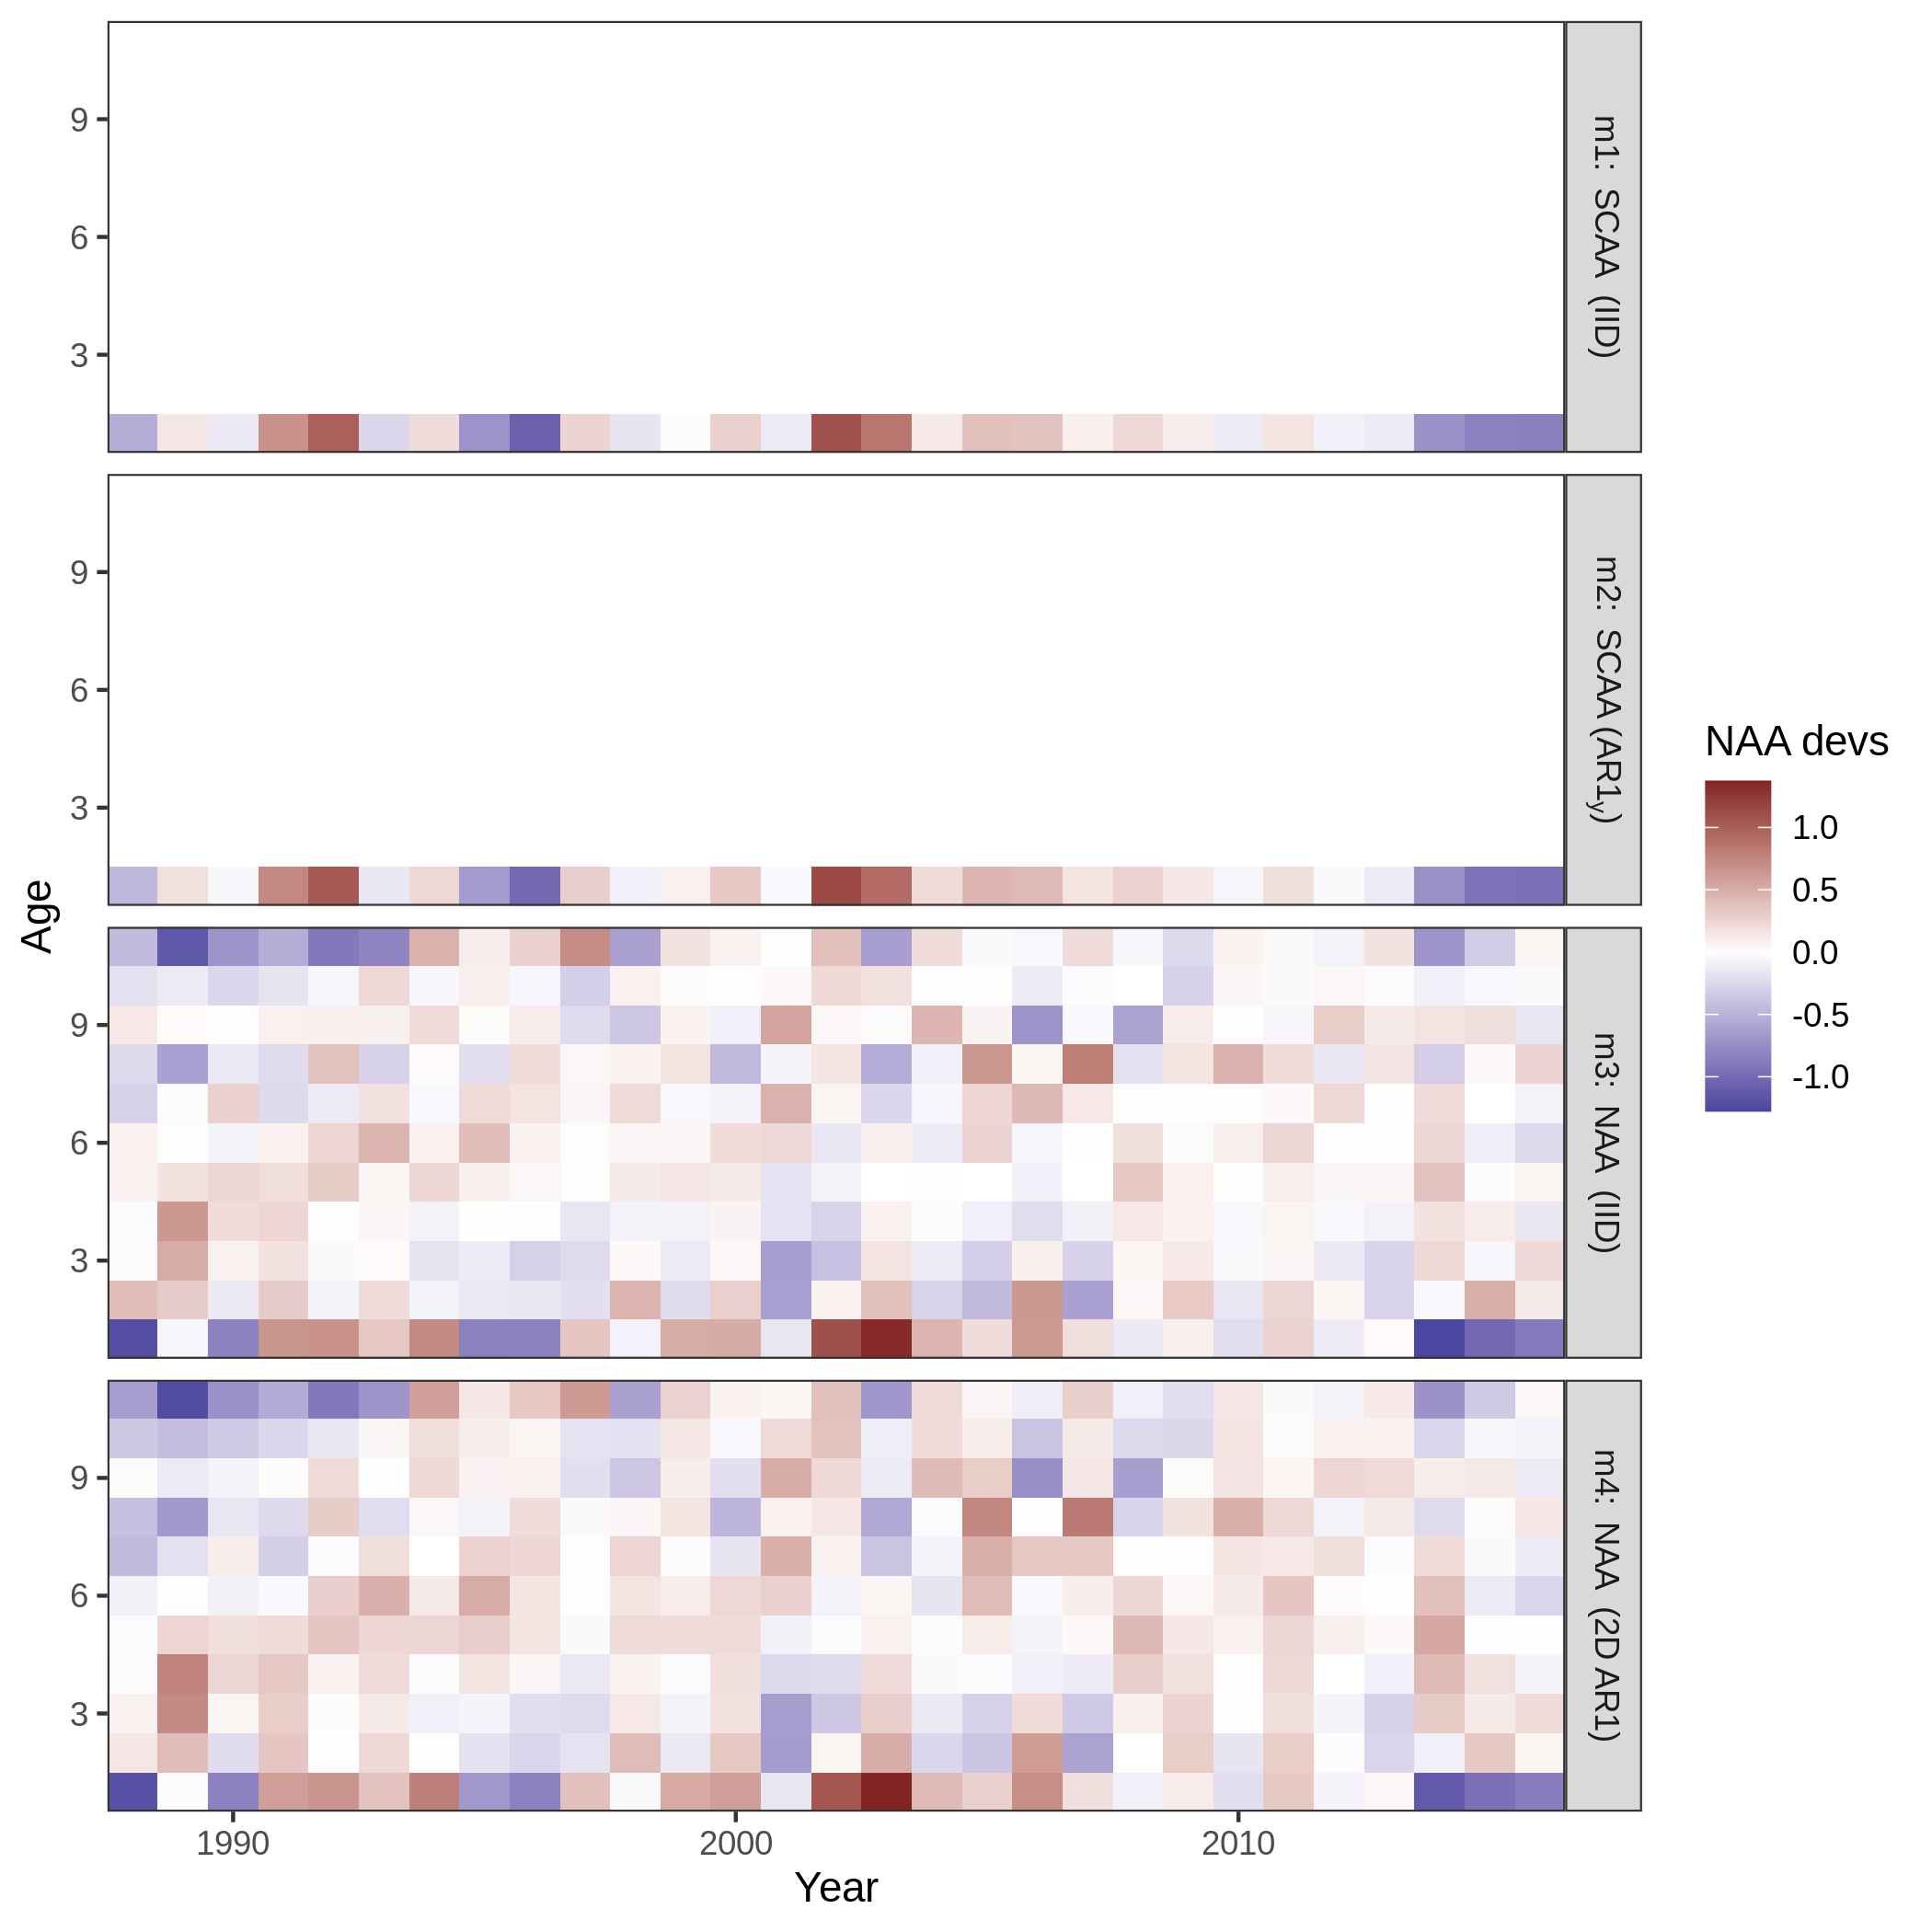
\includegraphics[width=6.5in]{/home/bstock/Documents/ms/wham-sim/plots/into_paper/8_REdevs_ICEherring_NAA} 

}

\caption{Survival deviations estimated for Icelandic herring using four models of numbers-at-age (NAA) random effects. m1 = only recruitment deviations are random effects (most similar to traditional statistical catch-at-age, SCAA), and deviations are independent and identically distributed (IID). m2 = as m1, but with autocorrelated recruitment deviations ($\text{AR1}_y$). m3 = all NAA deviations are IID random effects. m4 = as m3, but deviations are correlated by age and year (2D AR1).}\label{fig:devs-ICEherring-naa}
\end{figure}

\pagebreak

\begin{figure}

{\centering 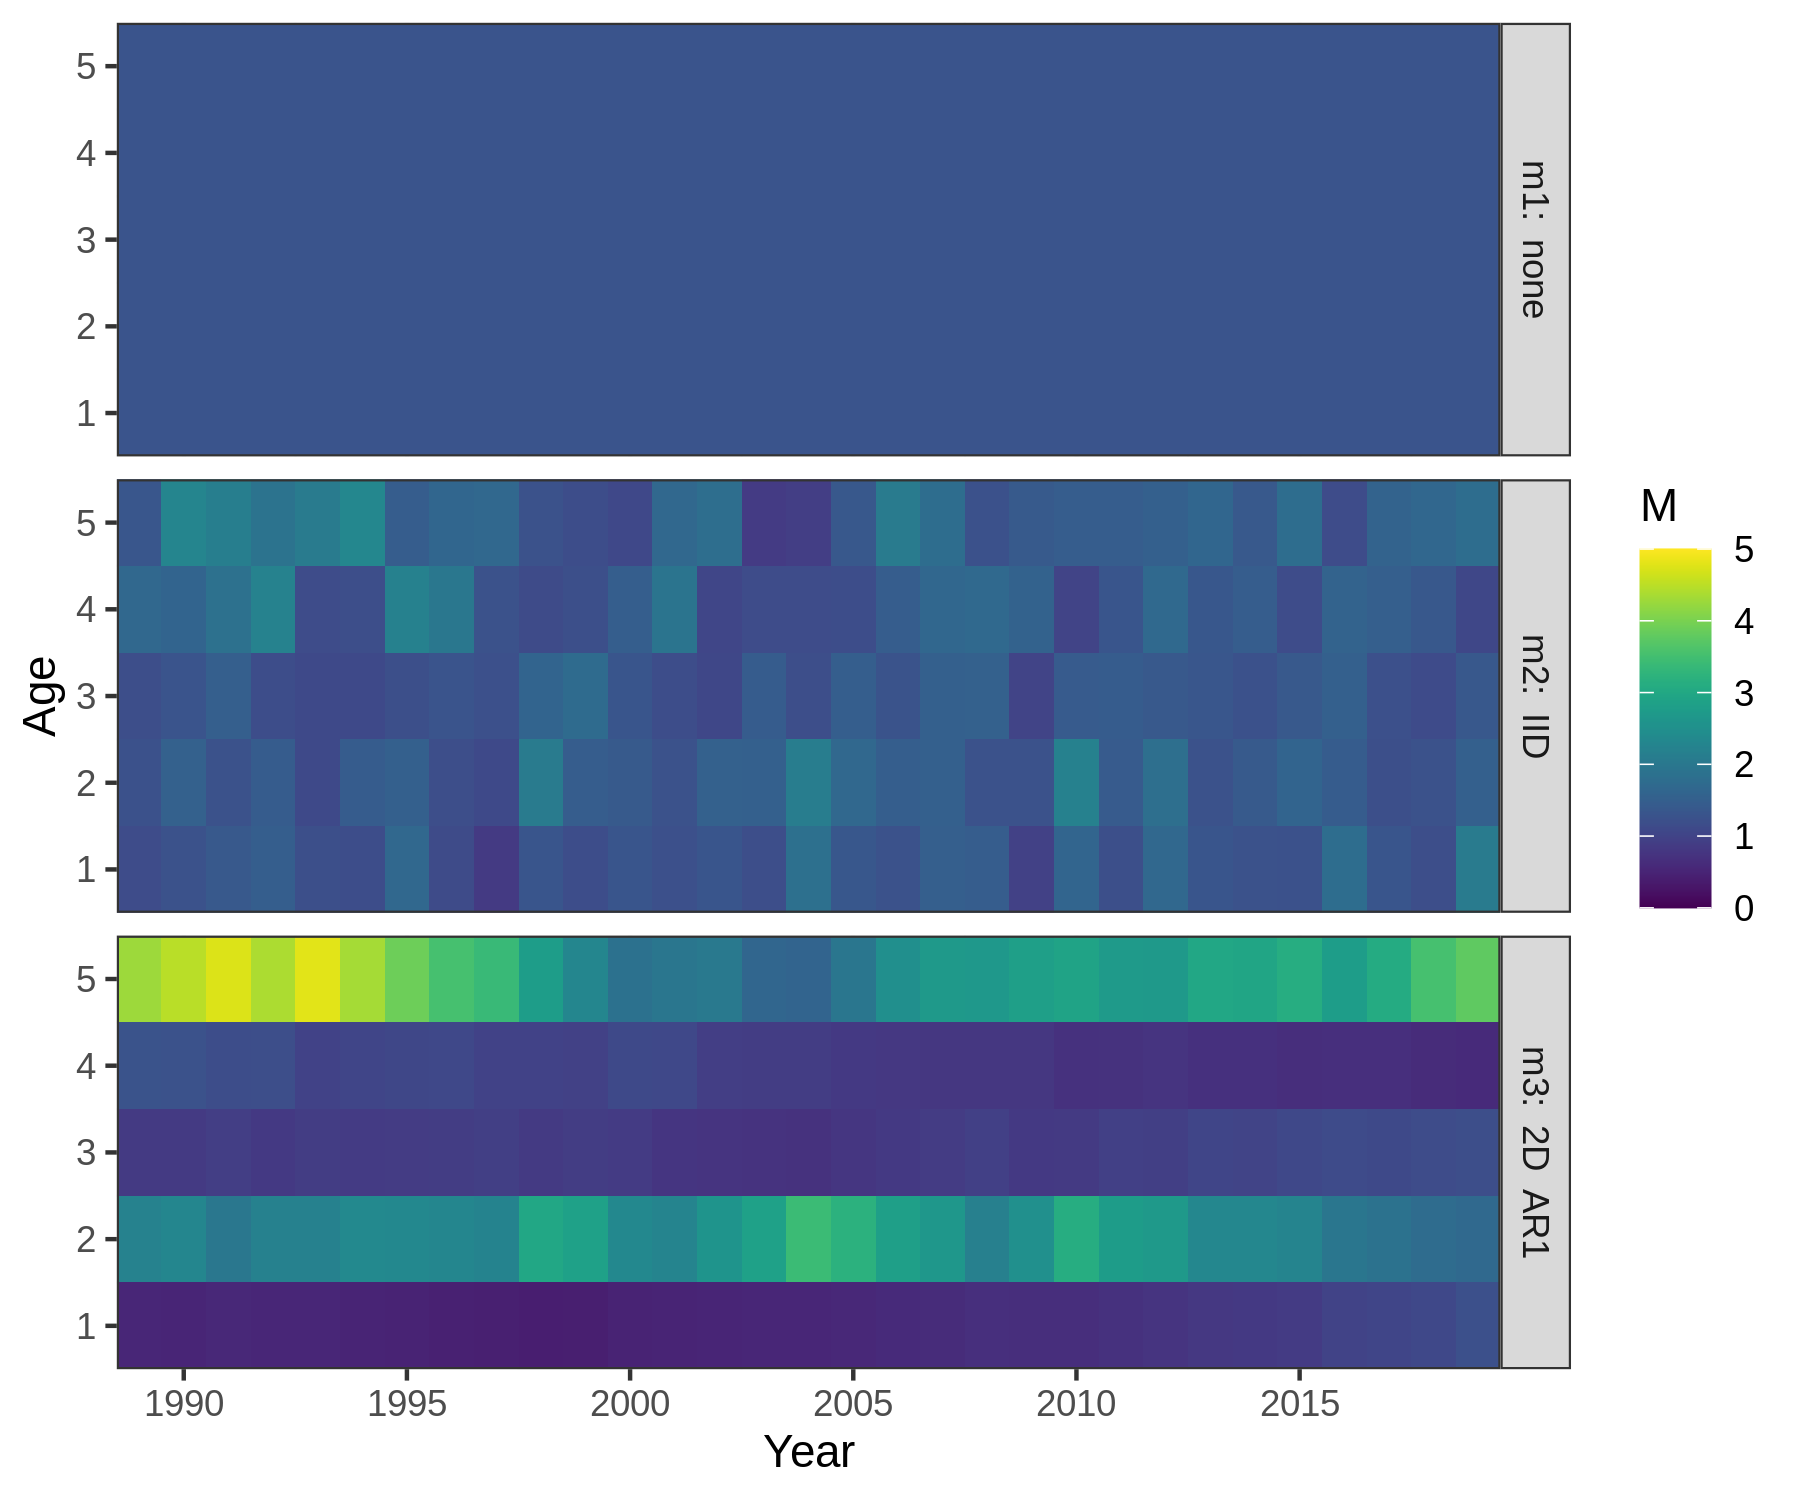
\includegraphics[width=6in]{/home/bstock/Documents/ms/wham-sim/plots/into_paper/8_REdevs_butterfish_M} 

}

\caption{Natural mortality (\textit{M}) estimated for butterfish using three random effects models. m1 = no random effects on \textit{M}. m2 = \textit{M} deviations are independent and identically distributed (IID). m3 = \textit{M} deviations are correlated by age and year (2D AR1).}\label{fig:devs-butterfish-m}
\end{figure}

\pagebreak

\begin{figure}

{\centering 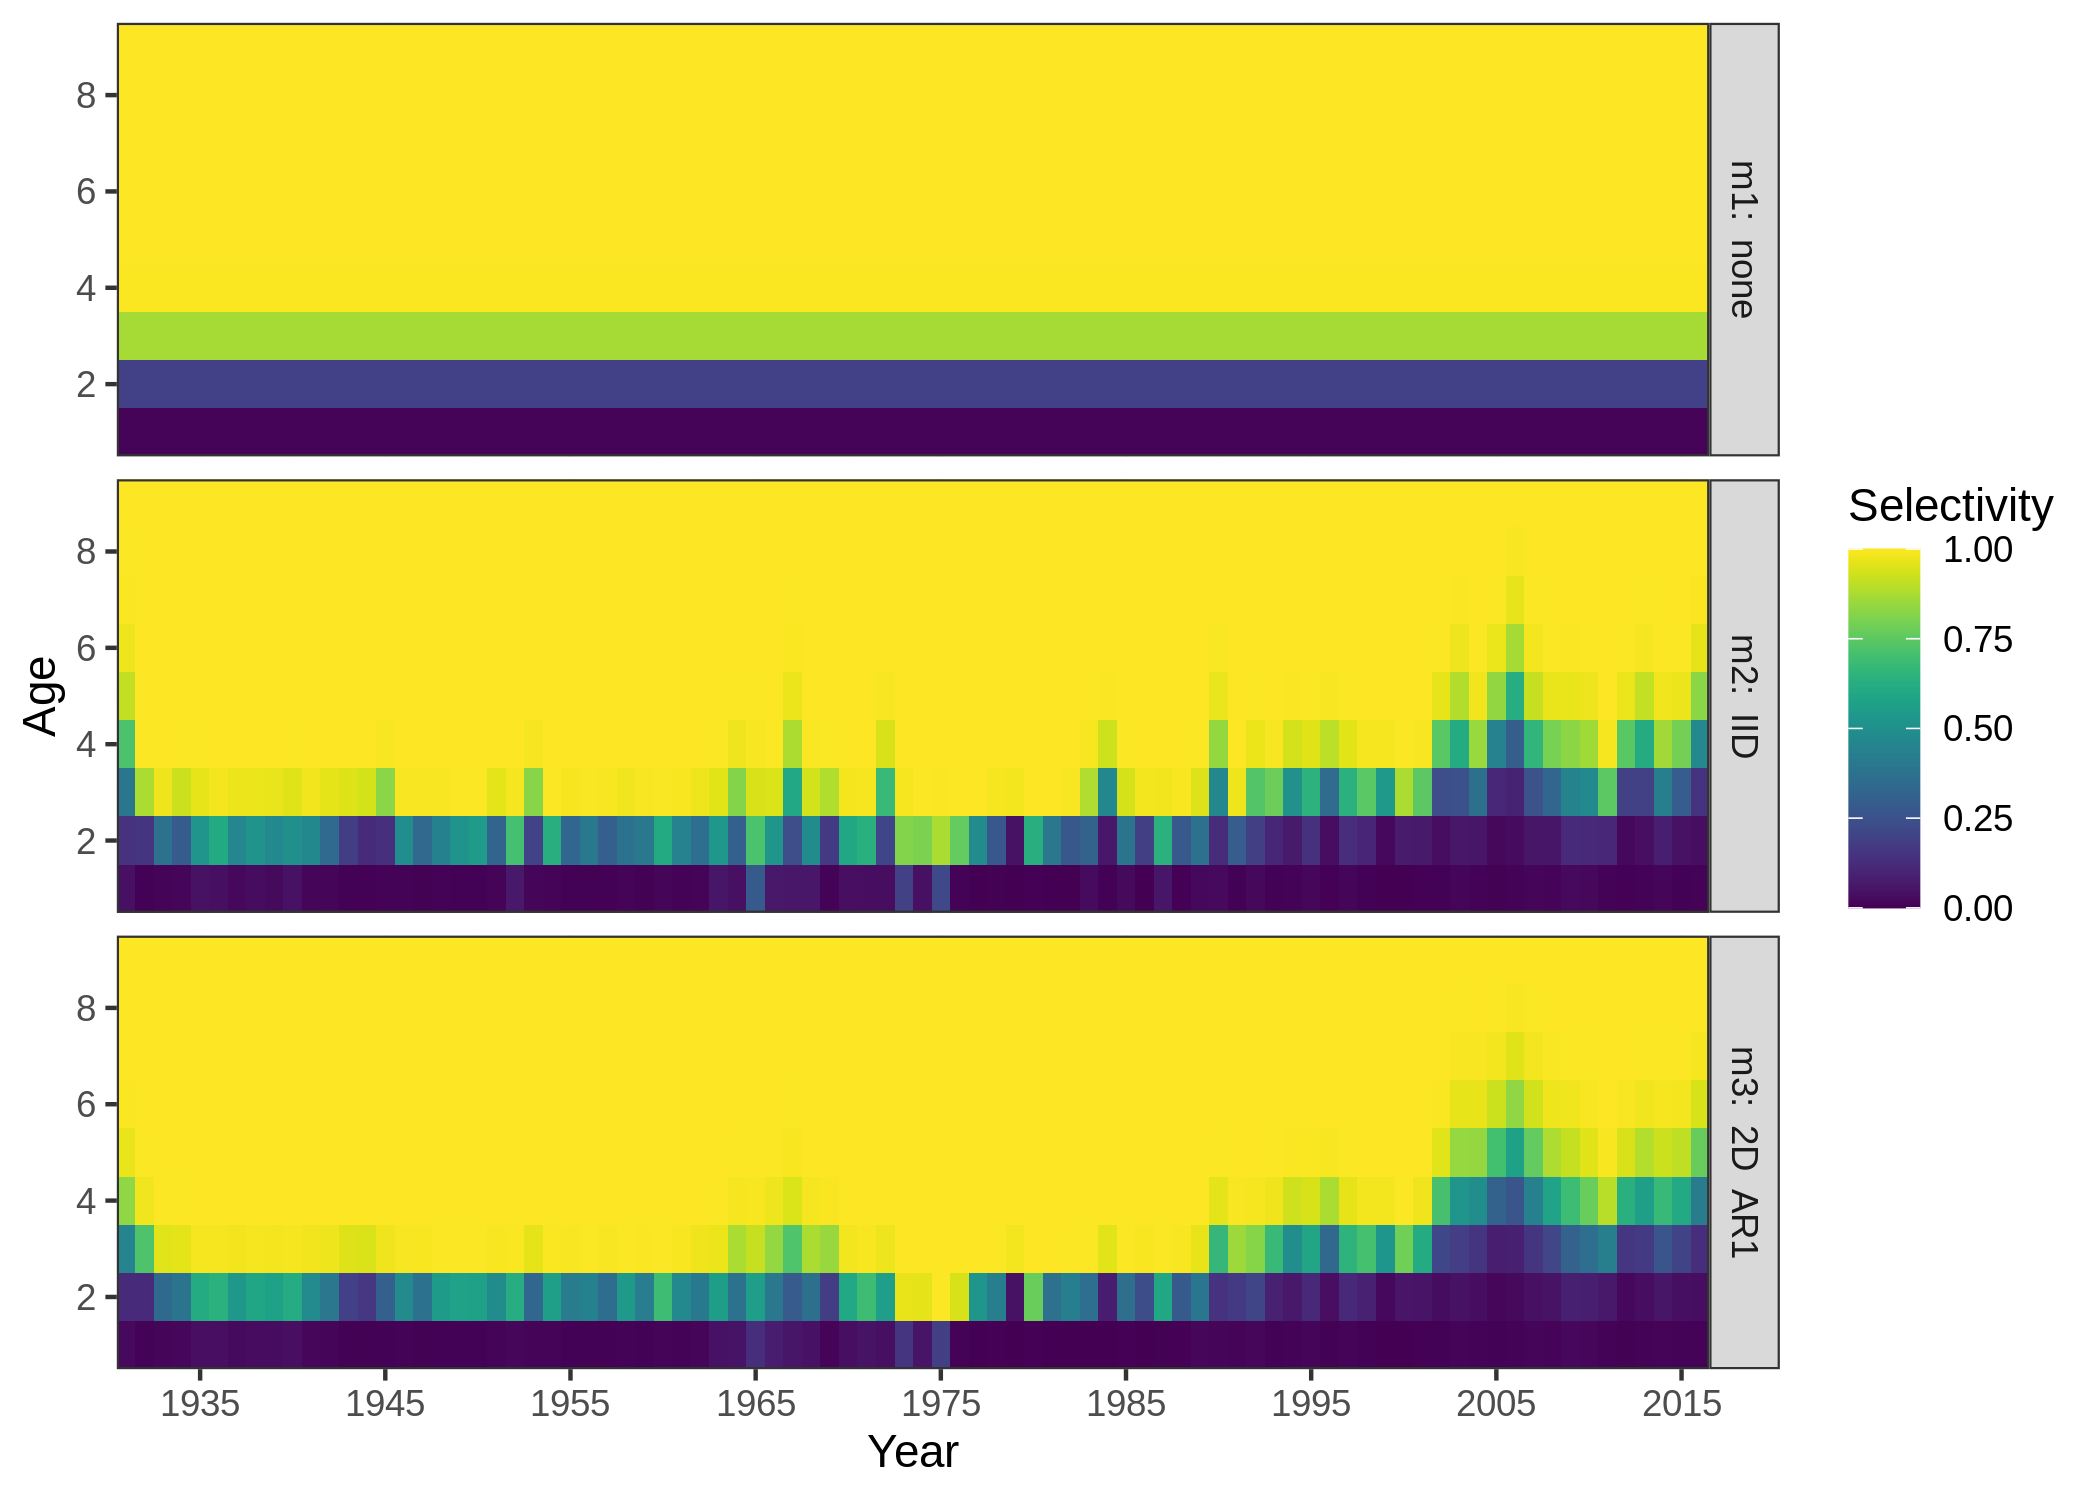
\includegraphics[width=6.5in]{/home/bstock/Documents/ms/wham-sim/plots/into_paper/8_REdevs_GBhaddock_sel} 

}

\caption{Selectivity estimated for Georges Bank haddock using three random effects models. m1 = no random effects (constant logistic selectivity). m2 = selectivity deviations are independent and identically distributed (IID). m3 = selectivity deviations are correlated by parameter and year (2D AR1).}\label{fig:devs-GBhaddock-sel}
\end{figure}

\pagebreak

\begin{figure}

{\centering 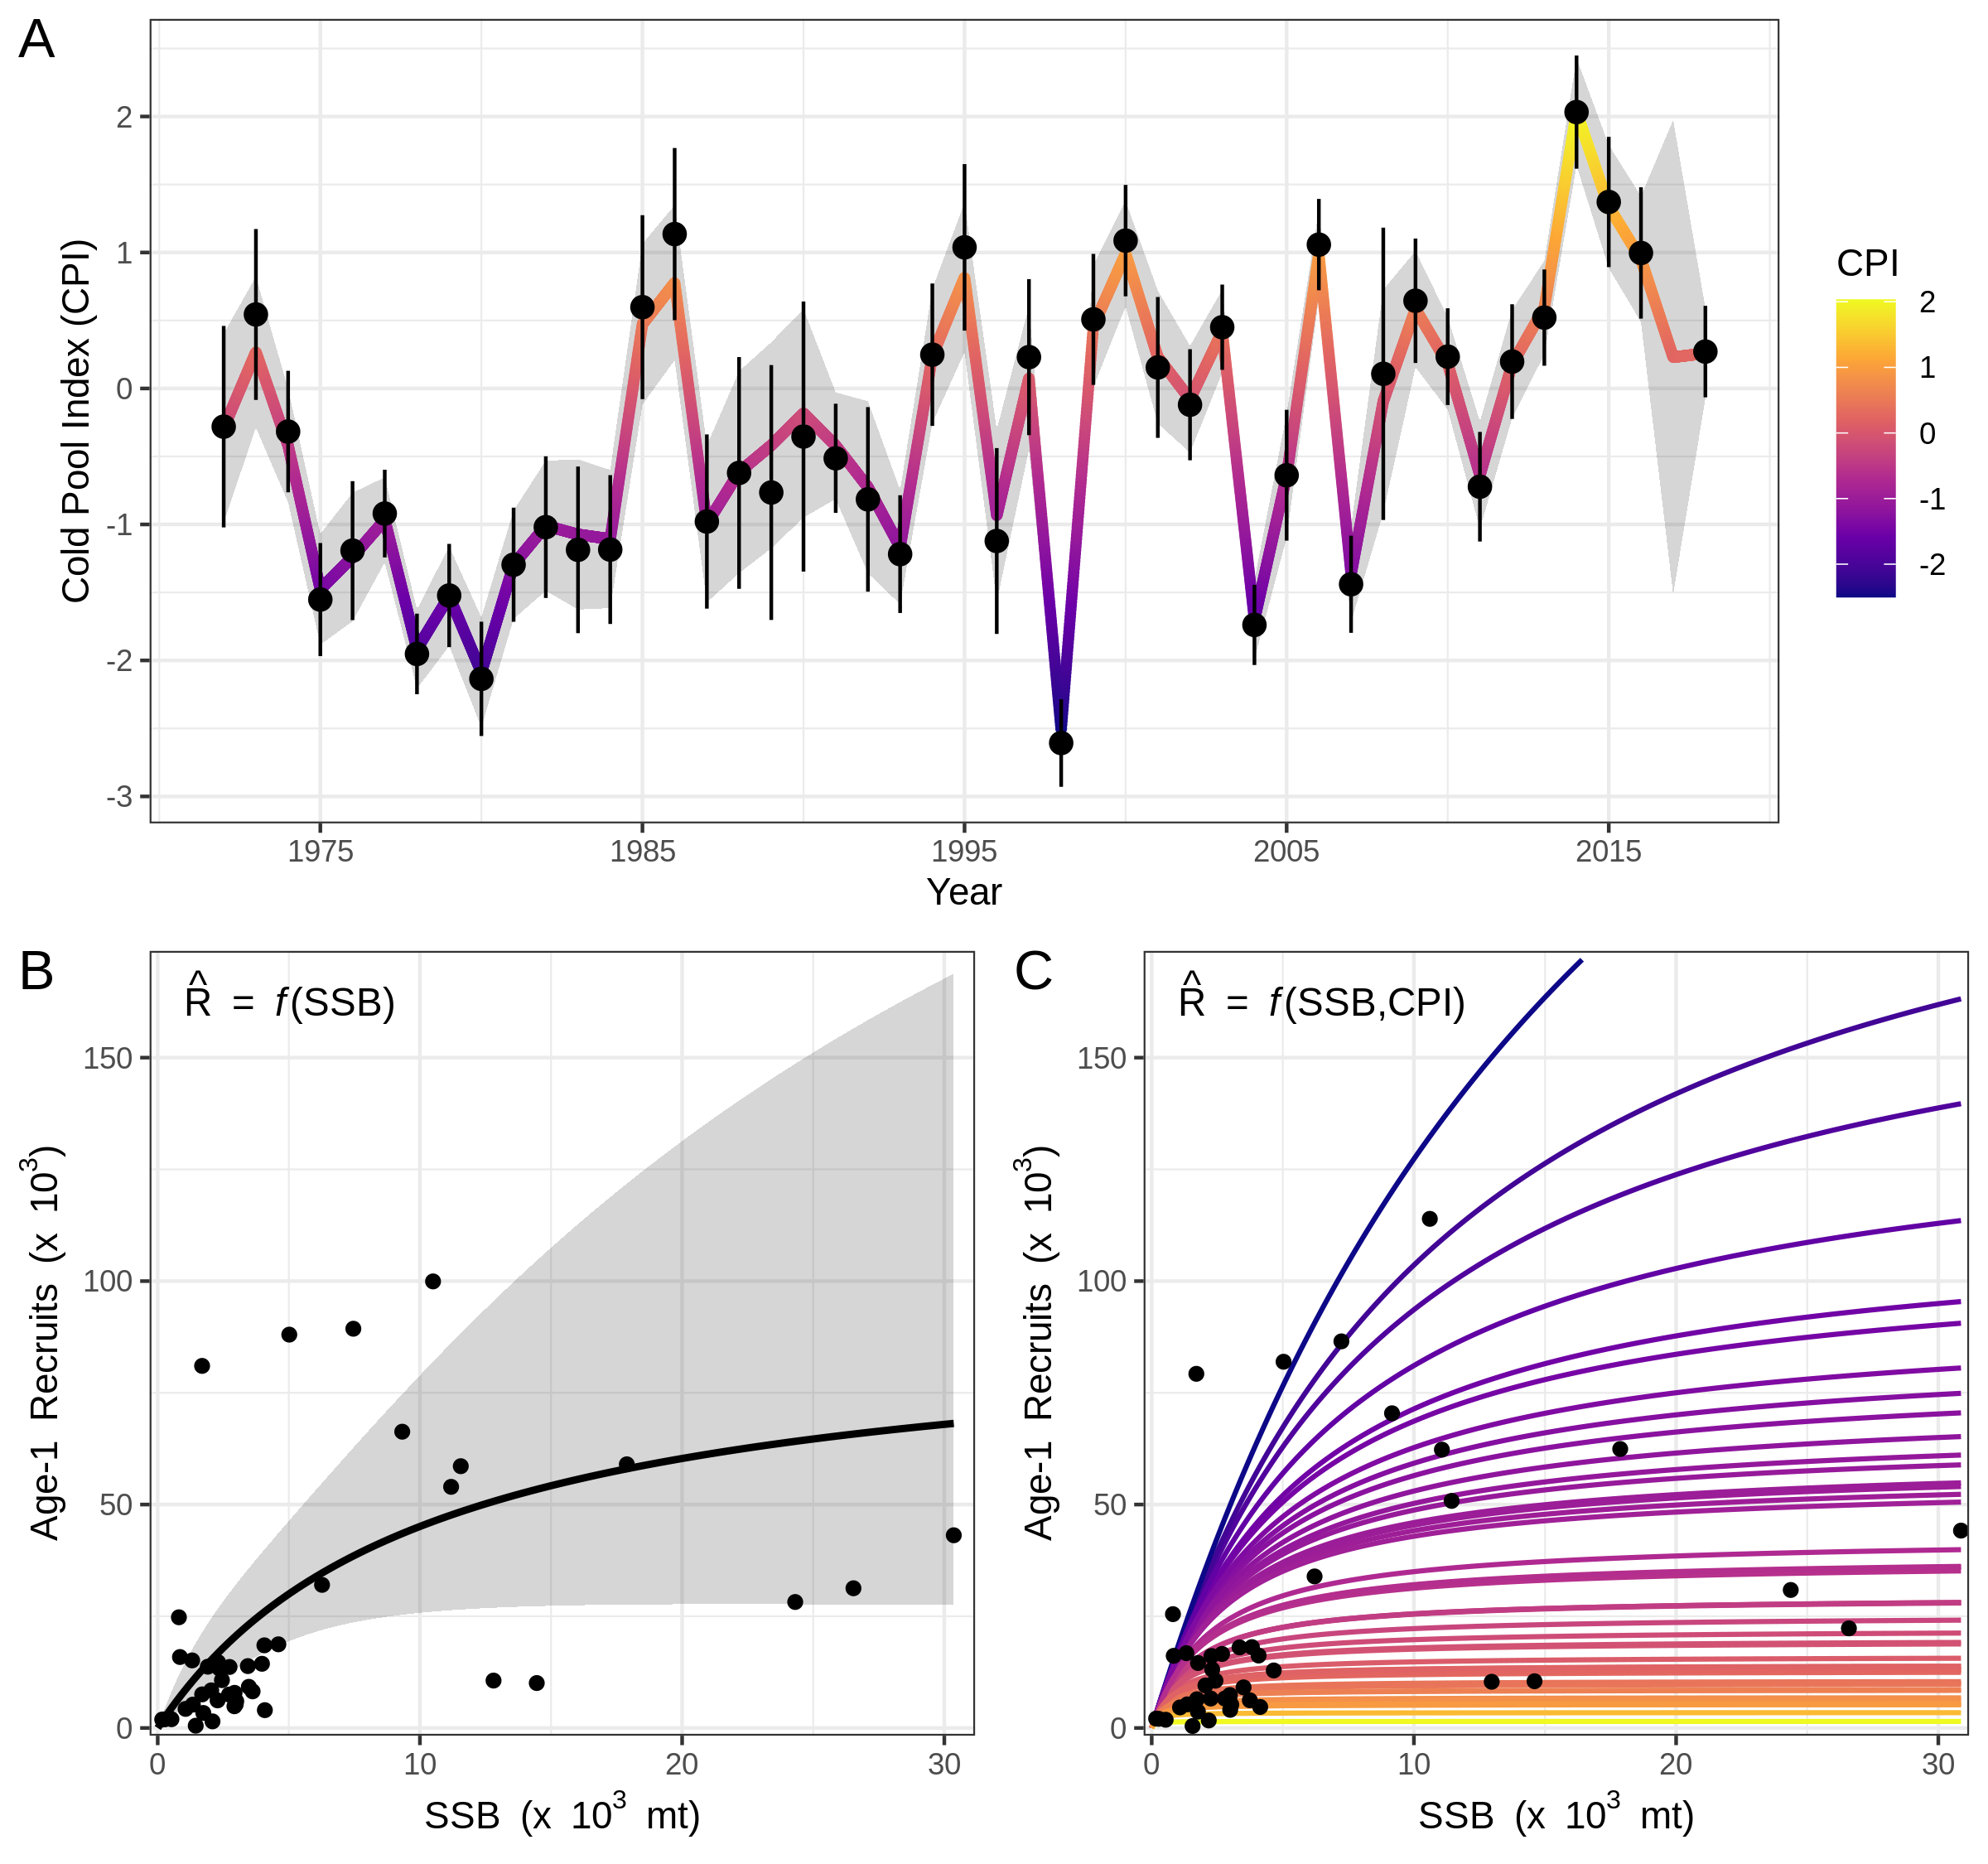
\includegraphics[width=6.5in]{/home/bstock/Documents/ms/wham-sim/plots/into_paper/8_CPI_Recruit_SNEMAYT_Ecov2} 

}

\caption{Beverton-Holt stock-recruit relationships fit for Southern New England-Mid Atlantic yellowtail flounder, with and without effects of the Cold Pool Index (CPI). A) CPI estimated from the model with lowest AIC (m4, AR1-linear). Points are observations with 95\% CI, and the line with shading is the model-estimated CPI with 95\% CI. Note the increased uncertainty surrounding the CPI estimate in 2017 (no observation). B) Estimates of spawning stock biomass (SSB), recruitment, and the stock-recruit function from the model without a CPI effect, m1. C) Estimates of SSB and recruitment from m4, with an effect of the CPI on $\beta$. Lines depict the expected stock-recruit relationship in each year $t$, given the CPI in year $t-1$ (color).}\label{fig:devs-SNEMAYT-ecov}
\end{figure}

\pagebreak

\begin{landscape}
\begin{figure}

{\centering 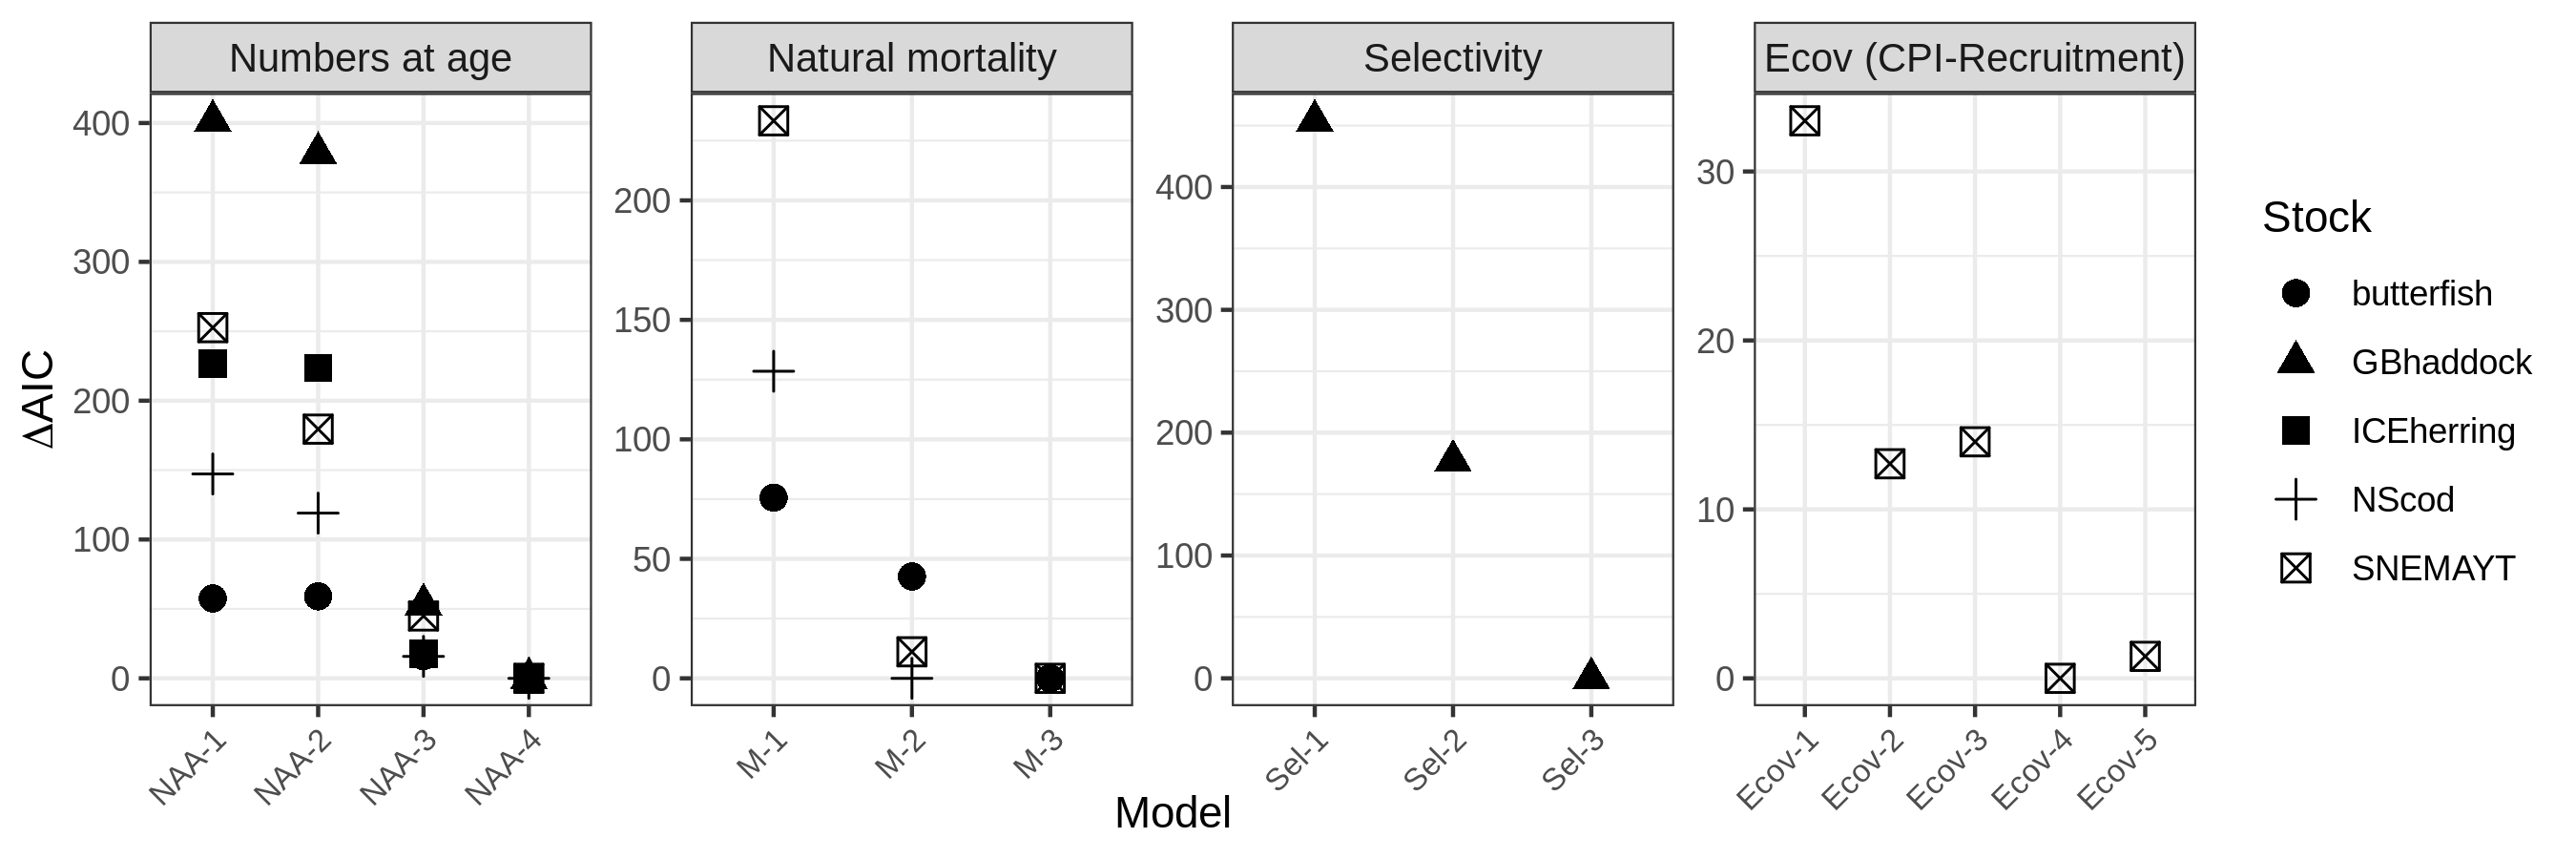
\includegraphics[width=8in]{/home/bstock/Documents/ms/wham-sim/plots/into_paper/daic} 

}

\caption{AIC differences by model and stock when fit to full datasets. Stock abbreviations: SNEMA yellowtail flounder (SNEMAYT), North Sea cod (NScod), Icelandic herring (ICEherring), and Georges Bank haddock (GBhaddock).}\label{fig:daic}
\end{figure}
\end{landscape}

\pagebreak

\begin{figure}

{\centering 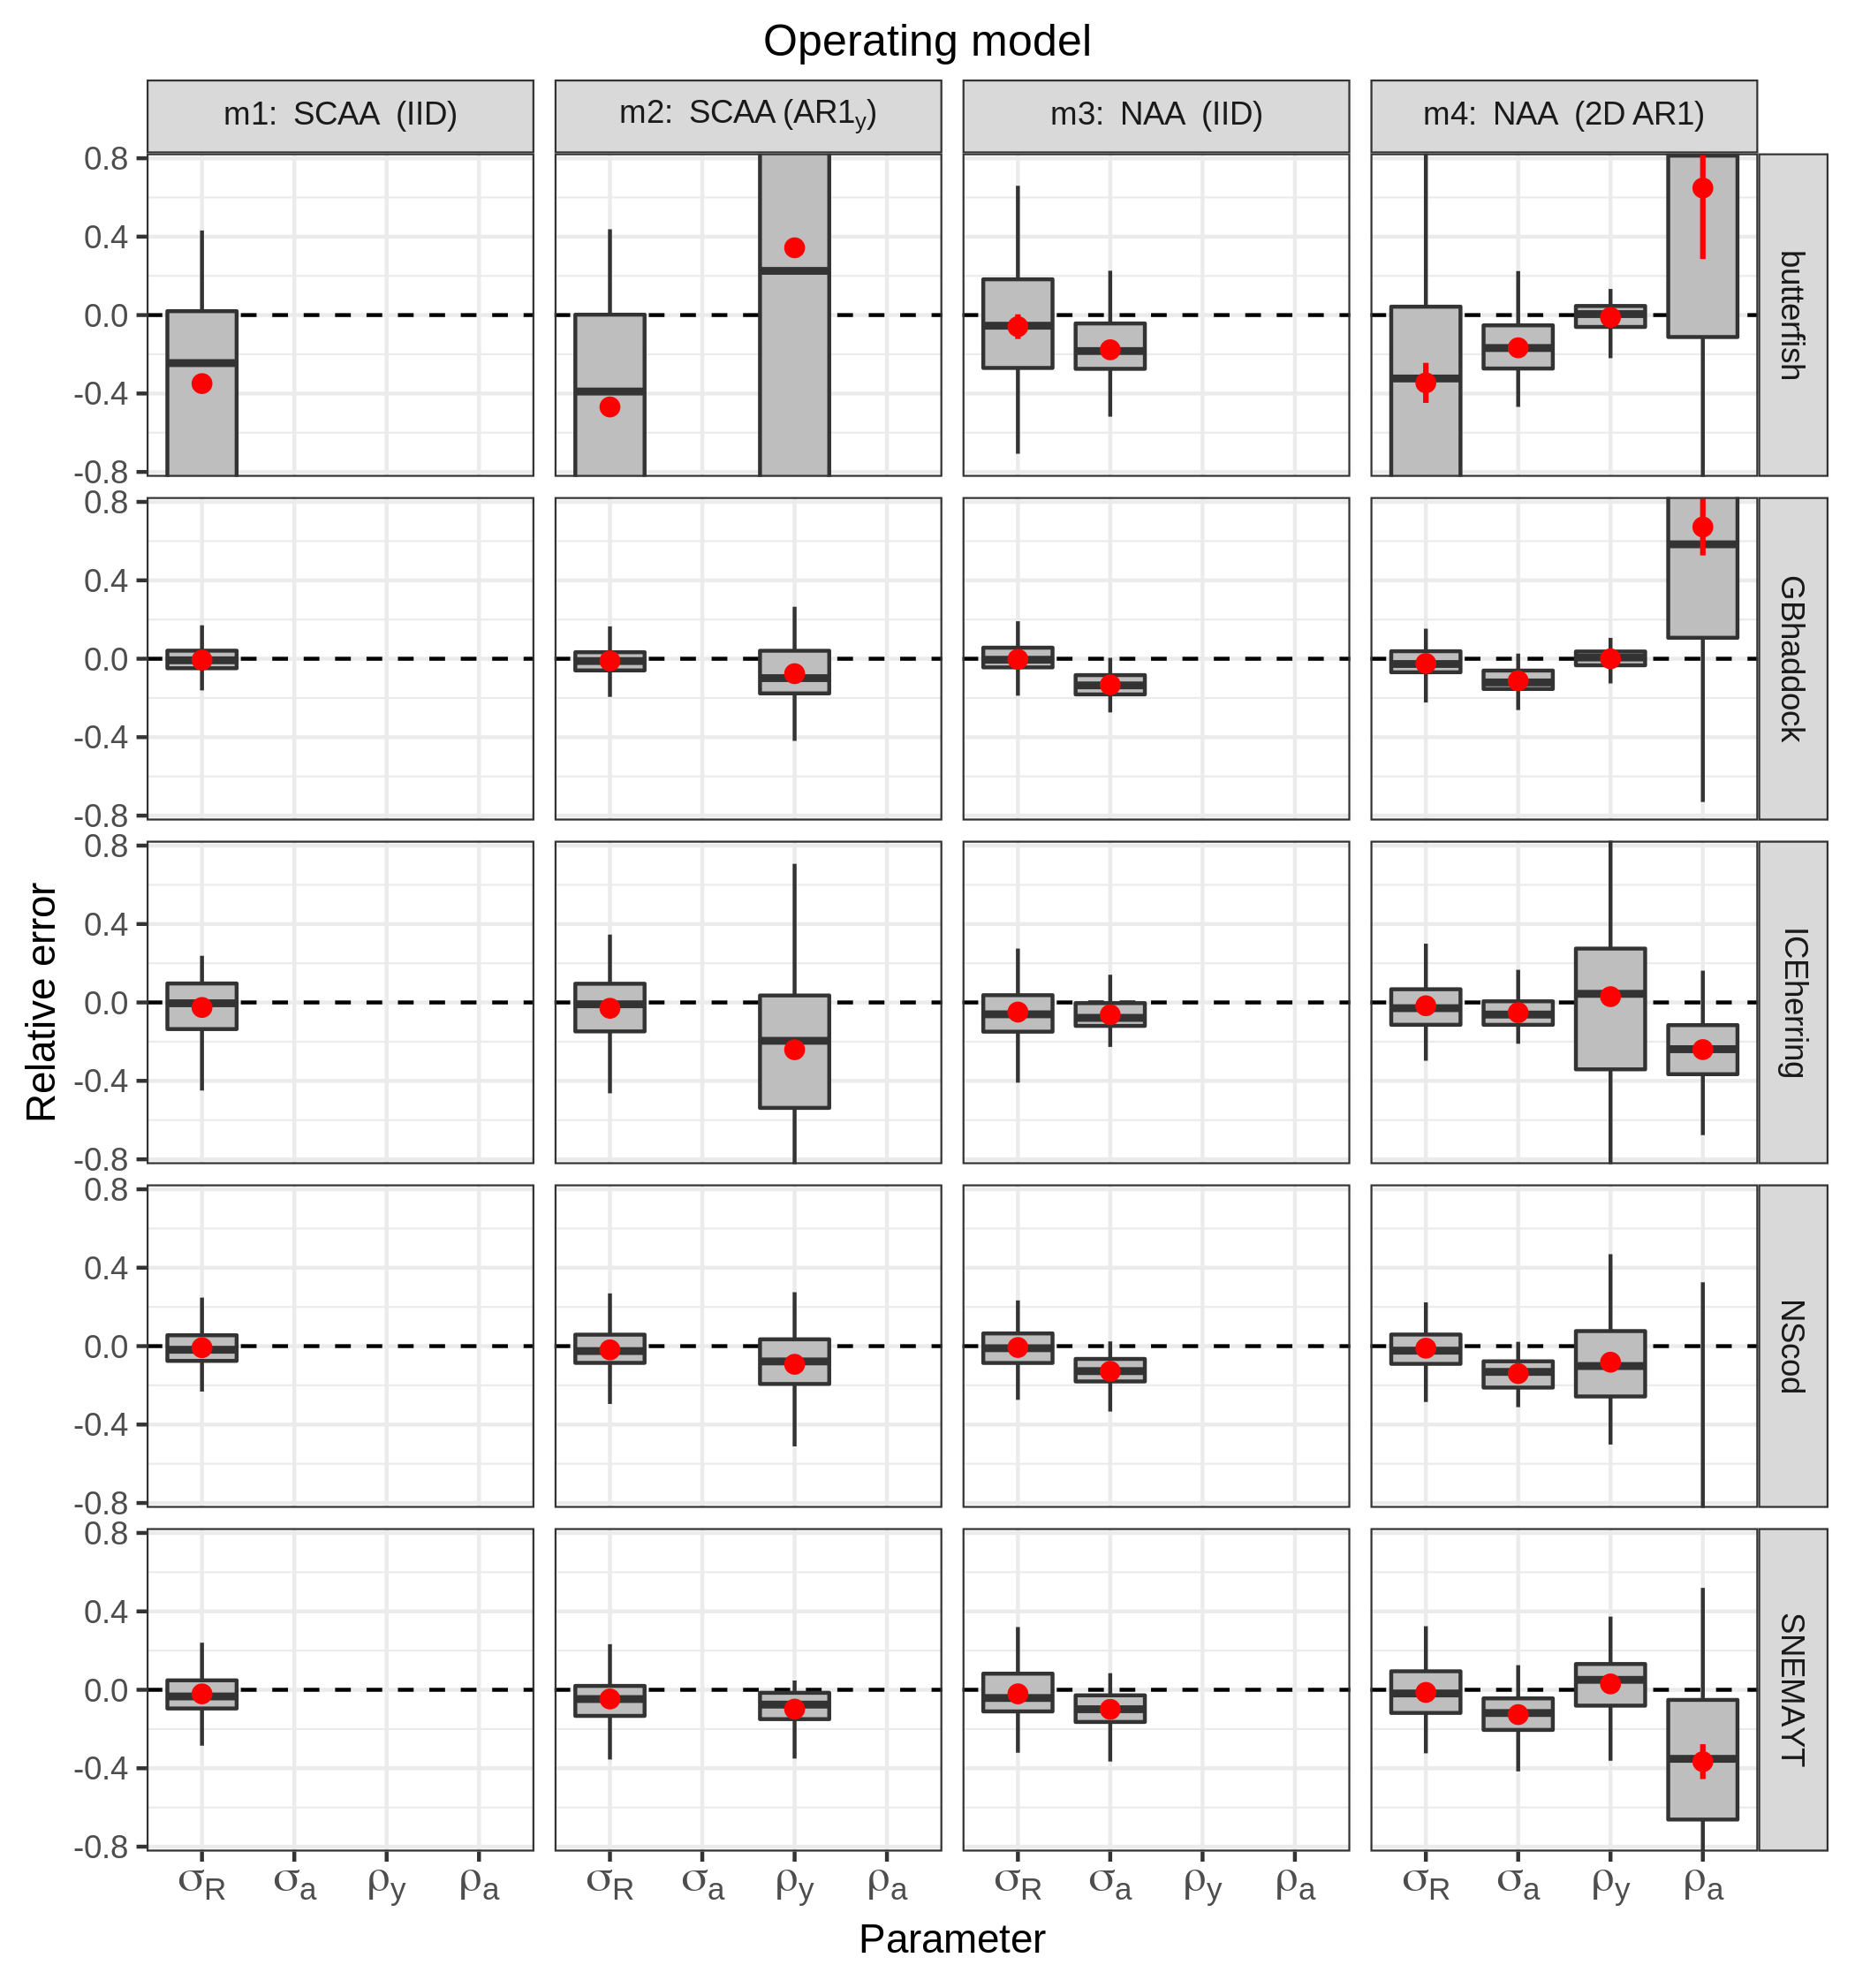
\includegraphics[width=6.5in]{/home/bstock/Documents/ms/wham-sim/plots/into_paper/estpar_NAA_OEPE} 

}

\caption{Relative error of parameters constraining numbers-at-age (NAA) random effects. Four models were used to simulate 100 datasets keeping fixed effect parameters constant, and then re-fit to each simulated dataset. m1 = only recruitment deviations are random effects (most similar to traditional statistical catch-at-age, SCAA), and deviations are independent and identically distributed (IID). m2 = as m1, but with autocorrelated recruitment deviations ($\text{AR1}_y$). m3 = all NAA deviations are IID random effects. m4 = as m3, but deviations are correlated by age and year (2D AR1). Relative error was calculated as $\frac{\hat{\theta_i}}{\theta} - 1$, where $\hat{\theta_i}$ was the estimate in simulation $i$ for parameter $\theta$, and $\theta$ was the true value (estimate from original dataset). Red points and lines show median relative error with 95\% CI.}\label{fig:estpar-naa}
\end{figure}

\pagebreak

\begin{figure}

{\centering 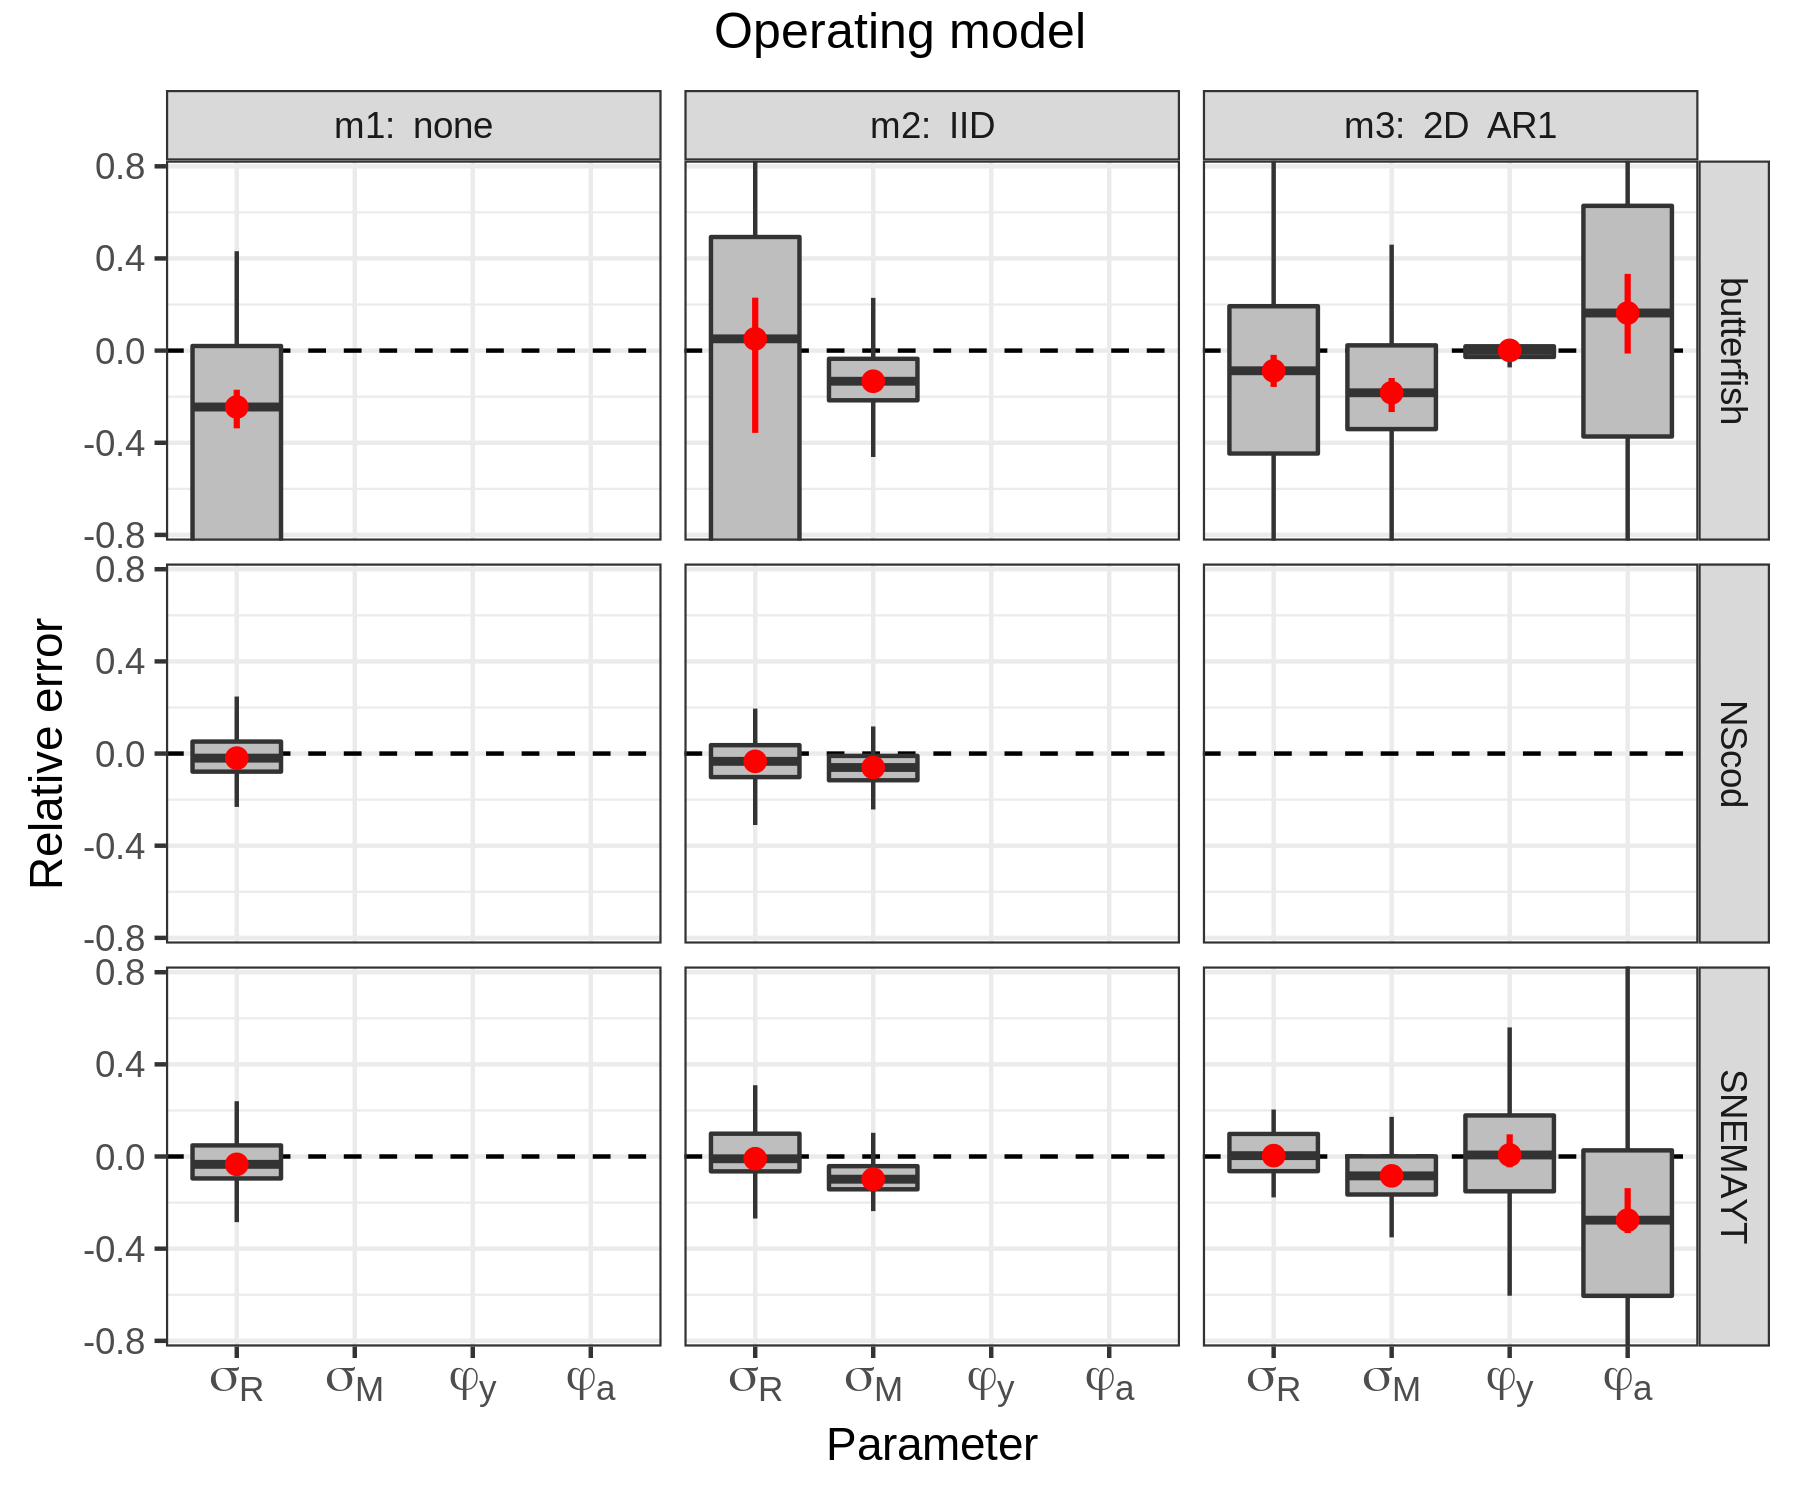
\includegraphics[width=6in]{/home/bstock/Documents/ms/wham-sim/plots/into_paper/estpar_M_4par_OEPE} 

}

\caption{Relative error of parameters constraining natural mortality (\textit{M}) random effects. Three models were used to simulate 100 datasets keeping fixed effect parameters constant, and then re-fit to each simulated dataset. m1 = no random effects on \textit{M}. m2 = \textit{M} deviations were independent and identically distributed (IID). m3 = \textit{M} deviations were correlated by age and year (2D AR1). Relative error was calculated as $\frac{\hat{\theta_i}}{\theta} - 1$, where $\hat{\theta_i}$ was the estimate in simulation $i$ for parameter $\theta$, and $\theta$ was the true value (estimate from original dataset). Red points and lines show median relative error with 95\% CI. Stock abbreviations: SNEMA yellowtail flounder (SNEMAYT) and North Sea cod (NScod, m3 did not converge).}\label{fig:estpar-m}
\end{figure}

\pagebreak

\begin{figure}

{\centering 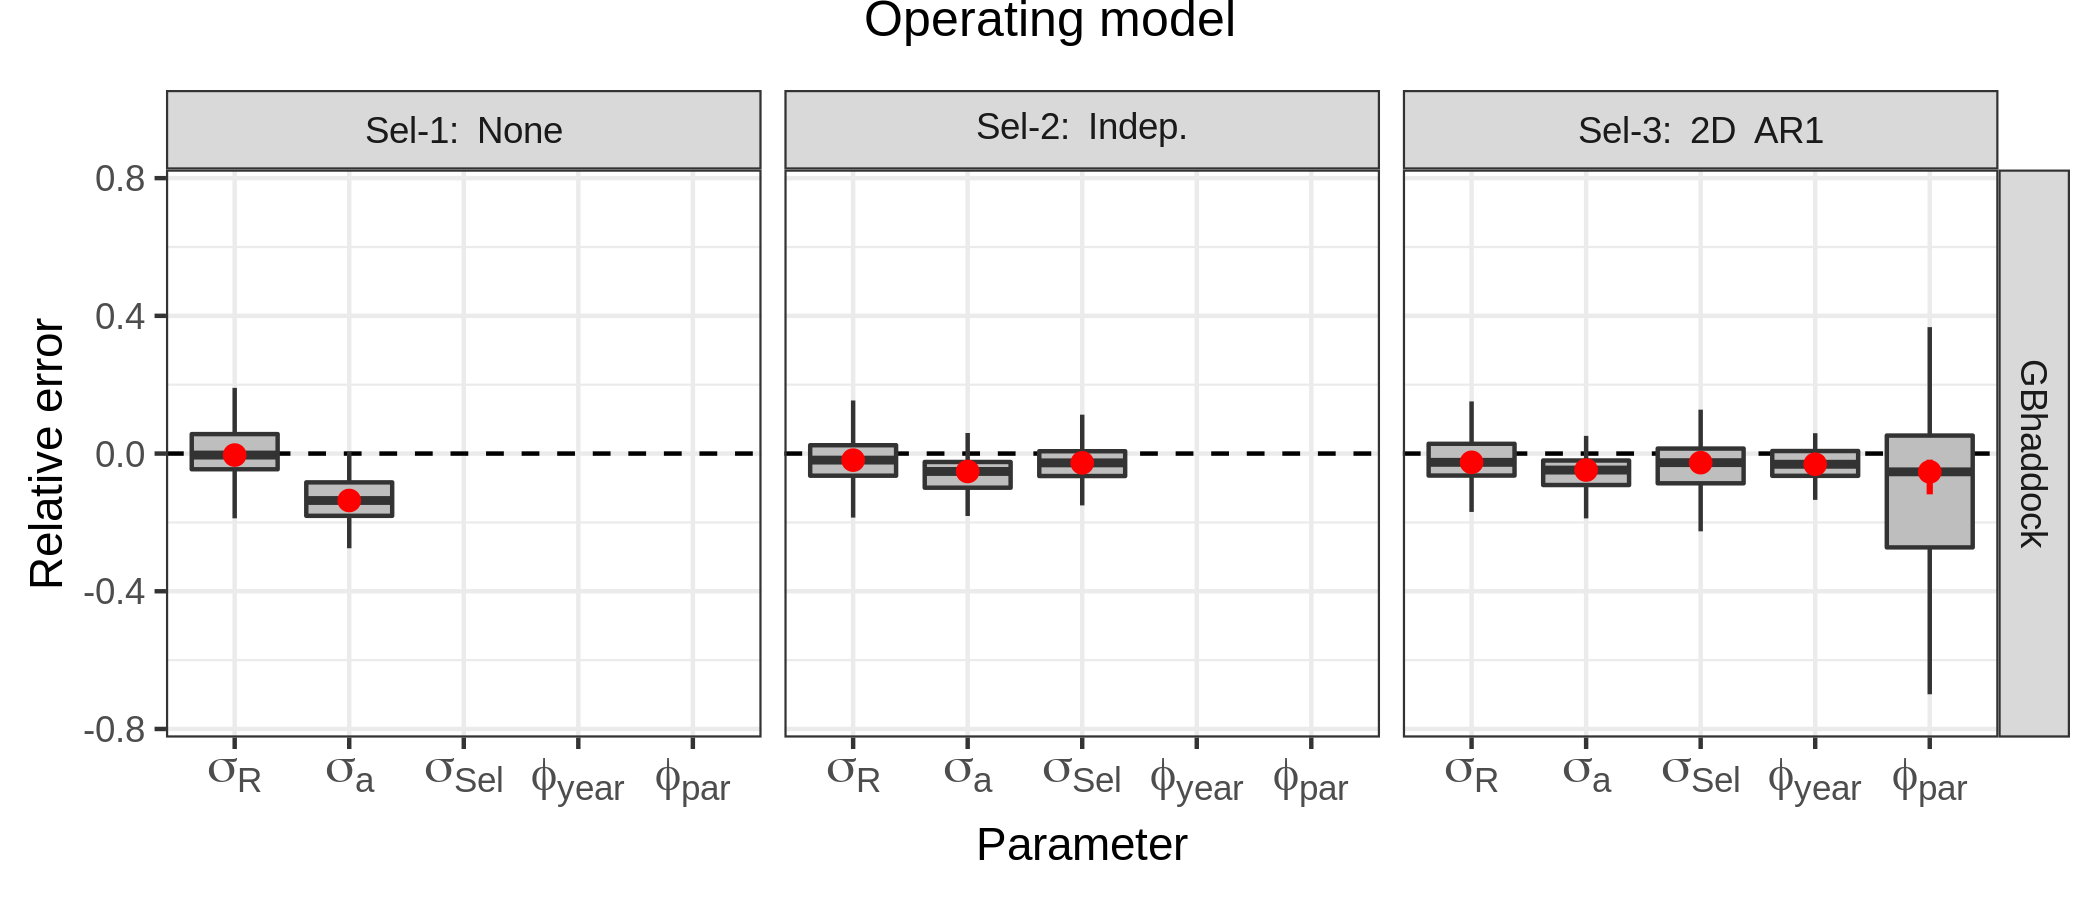
\includegraphics[width=6.5in]{/home/bstock/Documents/ms/wham-sim/plots/into_paper/estpar_sel_OEPE} 

}

\caption{Relative error of parameters constraining selectivity random effects for Georges Bank haddock (GBhaddock). Three models were used to simulate 100 datasets keeping fixed effect parameters constant, and then re-fit to each simulated dataset. m1 = no random effects (constant selectivity). m2 = selectivity deviations were independent and identically distributed (IID). m3 = selectivity deviations were correlated by parameter and year (2D AR1). Relative error was calculated as $\frac{\hat{\theta_i}}{\theta} - 1$, where $\hat{\theta_i}$ was the estimate in simulation $i$ for parameter $\theta$, and $\theta$ was the true value (estimate from original dataset). Red points and lines show median relative error with 95\% CI.}\label{fig:estpar-sel}
\end{figure}

\pagebreak

\begin{landscape}
\begin{figure}

{\centering 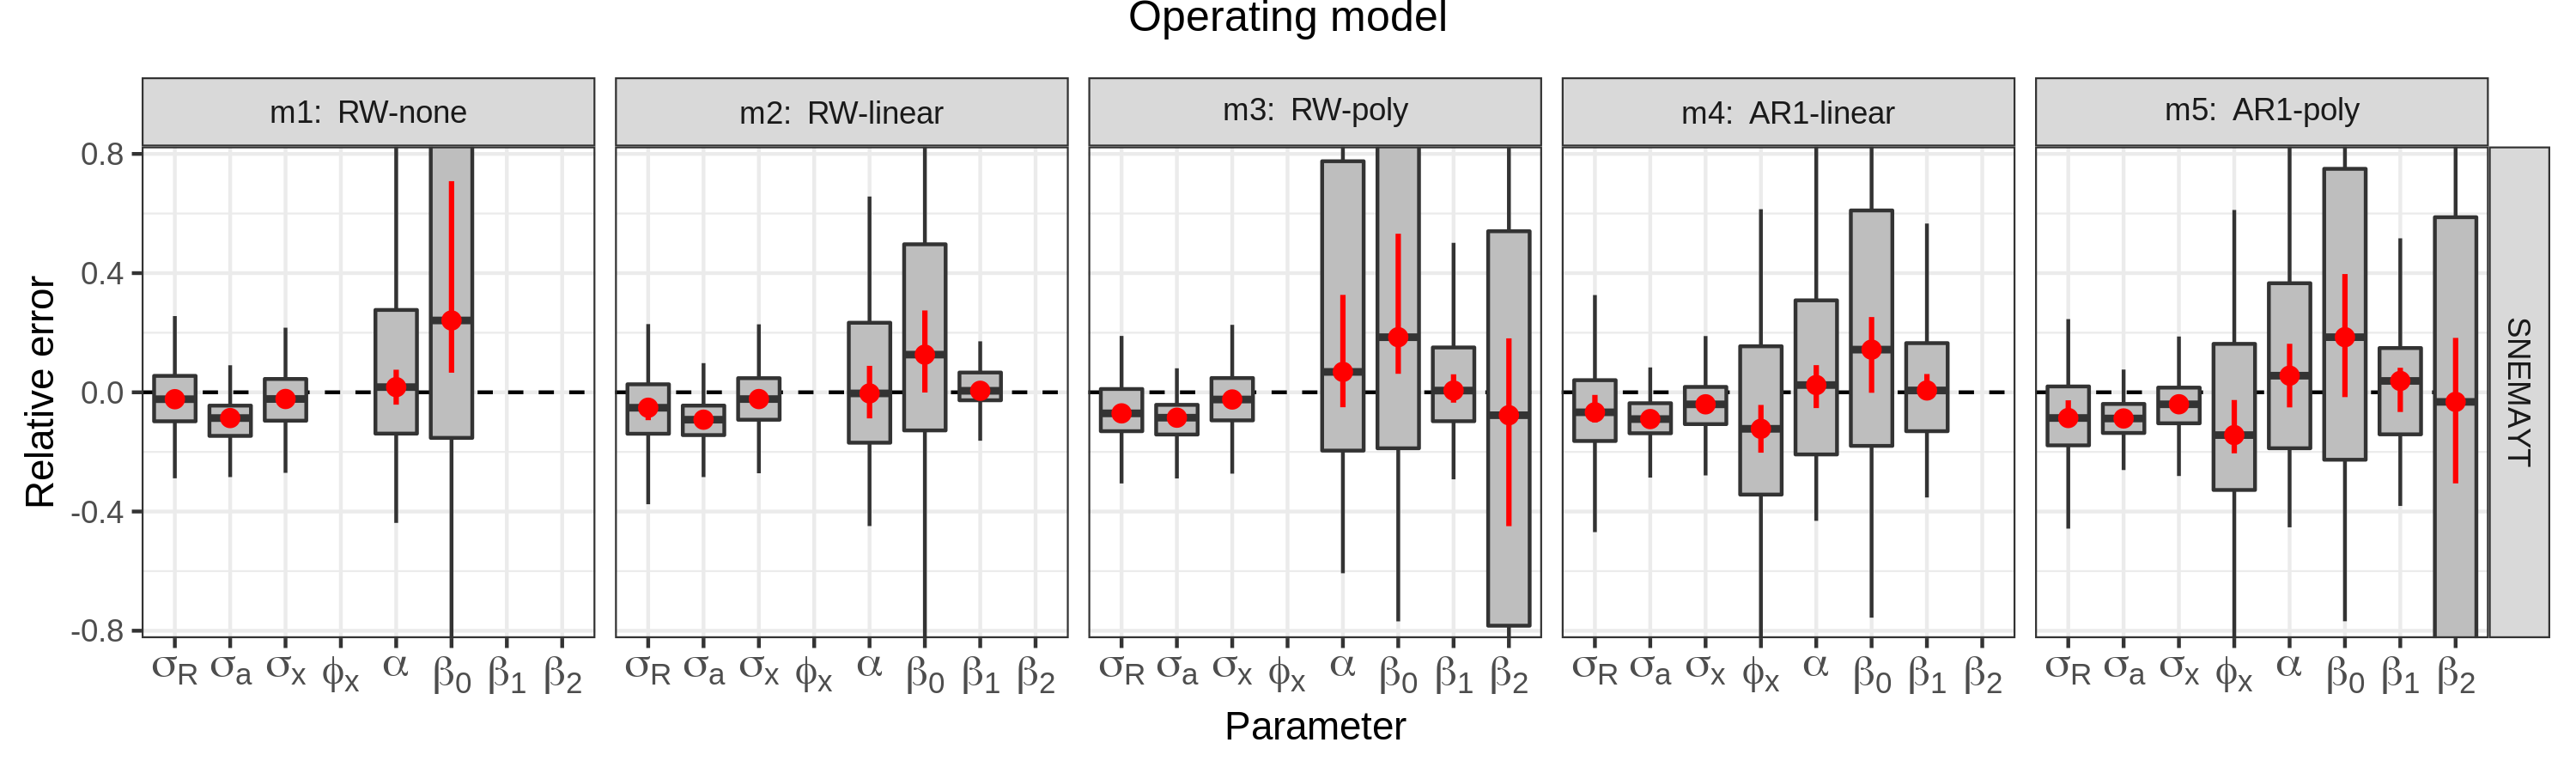
\includegraphics[width=9in]{/home/bstock/Documents/ms/wham-sim/plots/into_paper/estpar_Ecov2_OEPE} 

}

\caption{Relative error of parameters constraining variation in recruitment for Southern New England-Mid Atlantic yellowtail flounder (SNEMAYT). Five models were used to simulate 100 datasets keeping fixed effect parameters constant, and then re-fit to each simulated dataset. All models estimated recruitment using the Beverton-Holt function and included CPI effects on $\beta$: $\hat{R}_{t+1} = \frac{\alpha S_{t}}{1 + e^{\beta_0 + \beta_1 x_{t} + \beta_2 x^2_{t}} S_t}$. m1 = Cold Pool Index (CPI) modeled as a random walk (RW) with no effect on recruitment ($\beta_1 = \beta_2 = 0$). m2 = CPI as RW, linear effect on $\beta$. m3 = CPI as RW, 2nd order polynomial effect on $\beta$. m4 = CPI as AR1, linear effect. m5 = CPI as AR1, polynomial effect. Relative error was calculated as $\frac{\hat{\theta_i}}{\theta} - 1$, where $\hat{\theta_i}$ was the estimate in simulation $i$ for parameter $\theta$, and $\theta$ was the true value (estimate from original dataset). Red points and lines show median relative error with 95\% CI.}\label{fig:estpar-ecov}
\end{figure}
\end{landscape}

\pagebreak

\begin{figure}

{\centering 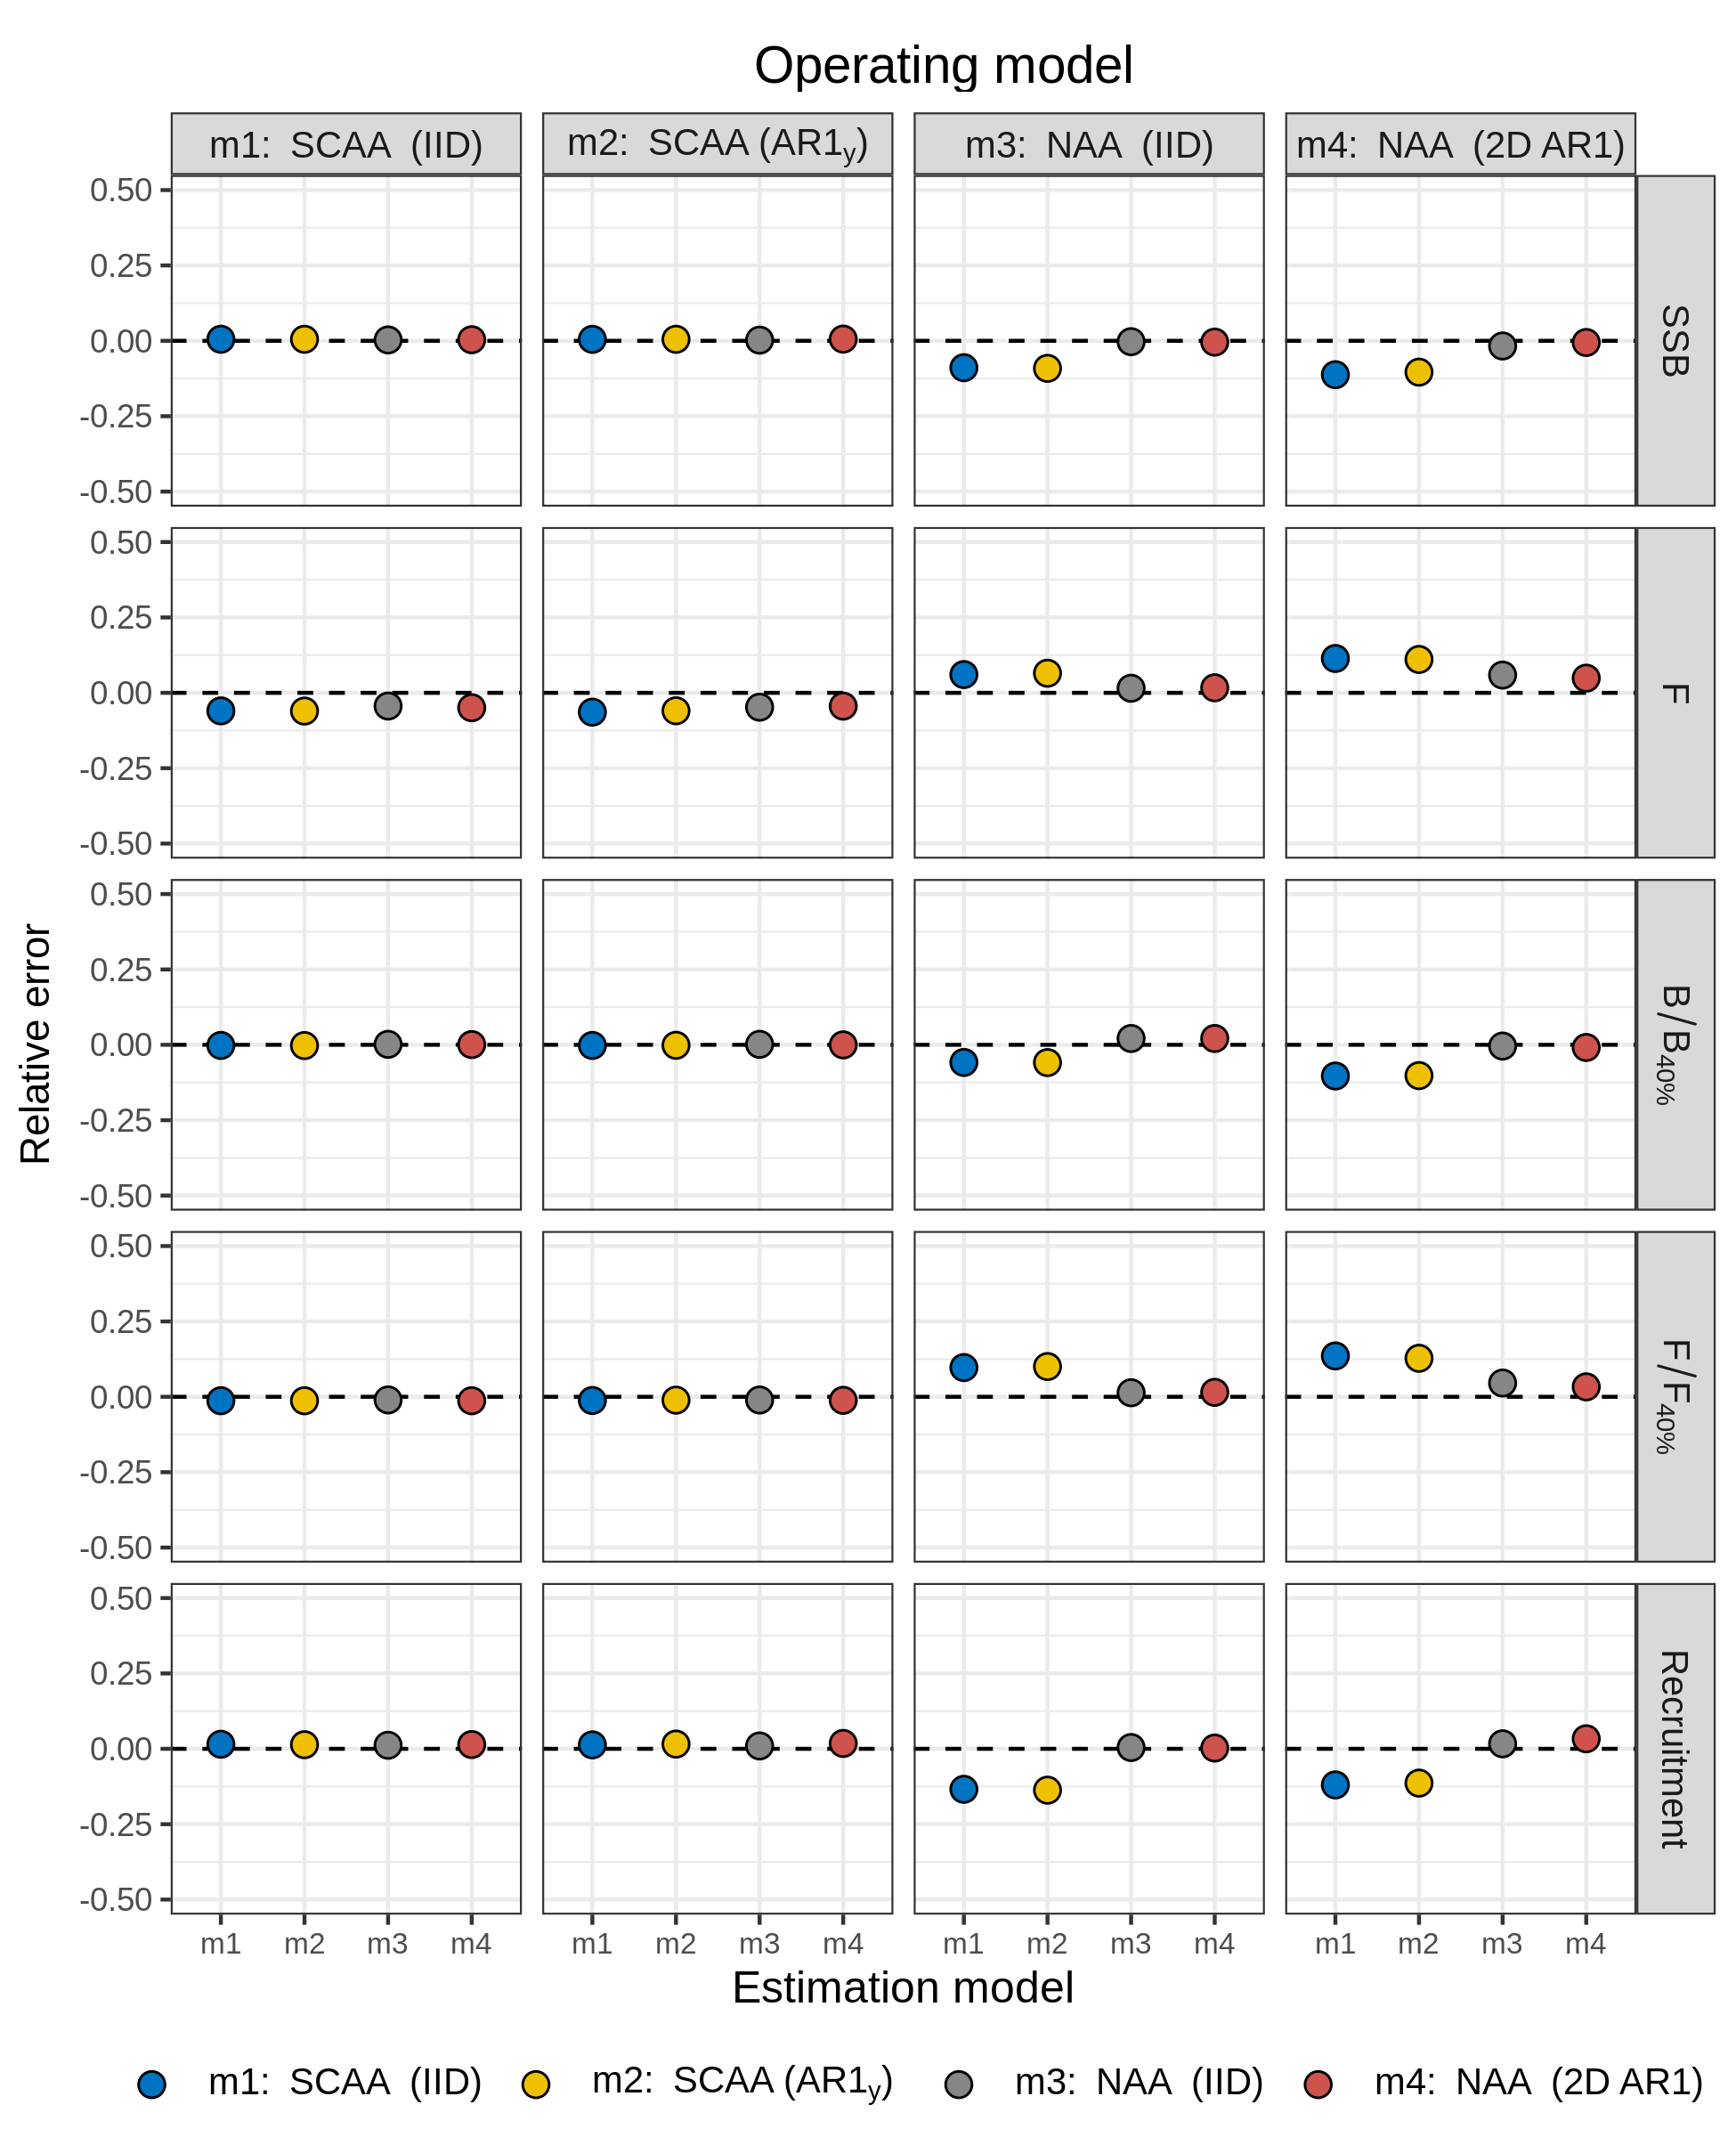
\includegraphics[width=6.5in]{/home/bstock/Documents/ms/wham-sim/plots/into_paper/0_ICEherring_NAA_medianCI_OEPE} 

}

\caption{Relative error of key quantities estimated for Icelandic herring using four models of numbers-at-age (NAA) random effects. m1 = only recruitment deviations are random effects (most similar to traditional statistical catch-at-age, SCAA), and deviations are independent and identically distributed (IID). m2 = as m1, but with autocorrelated recruitment deviations ($\text{AR1}_y$). m3 = all NAA deviations are IID random effects. m4 = as m3, but deviations are correlated by age and year (2D AR1).}\label{fig:rel-error-ICEherring-naa}
\end{figure}

\pagebreak

\begin{figure}

{\centering 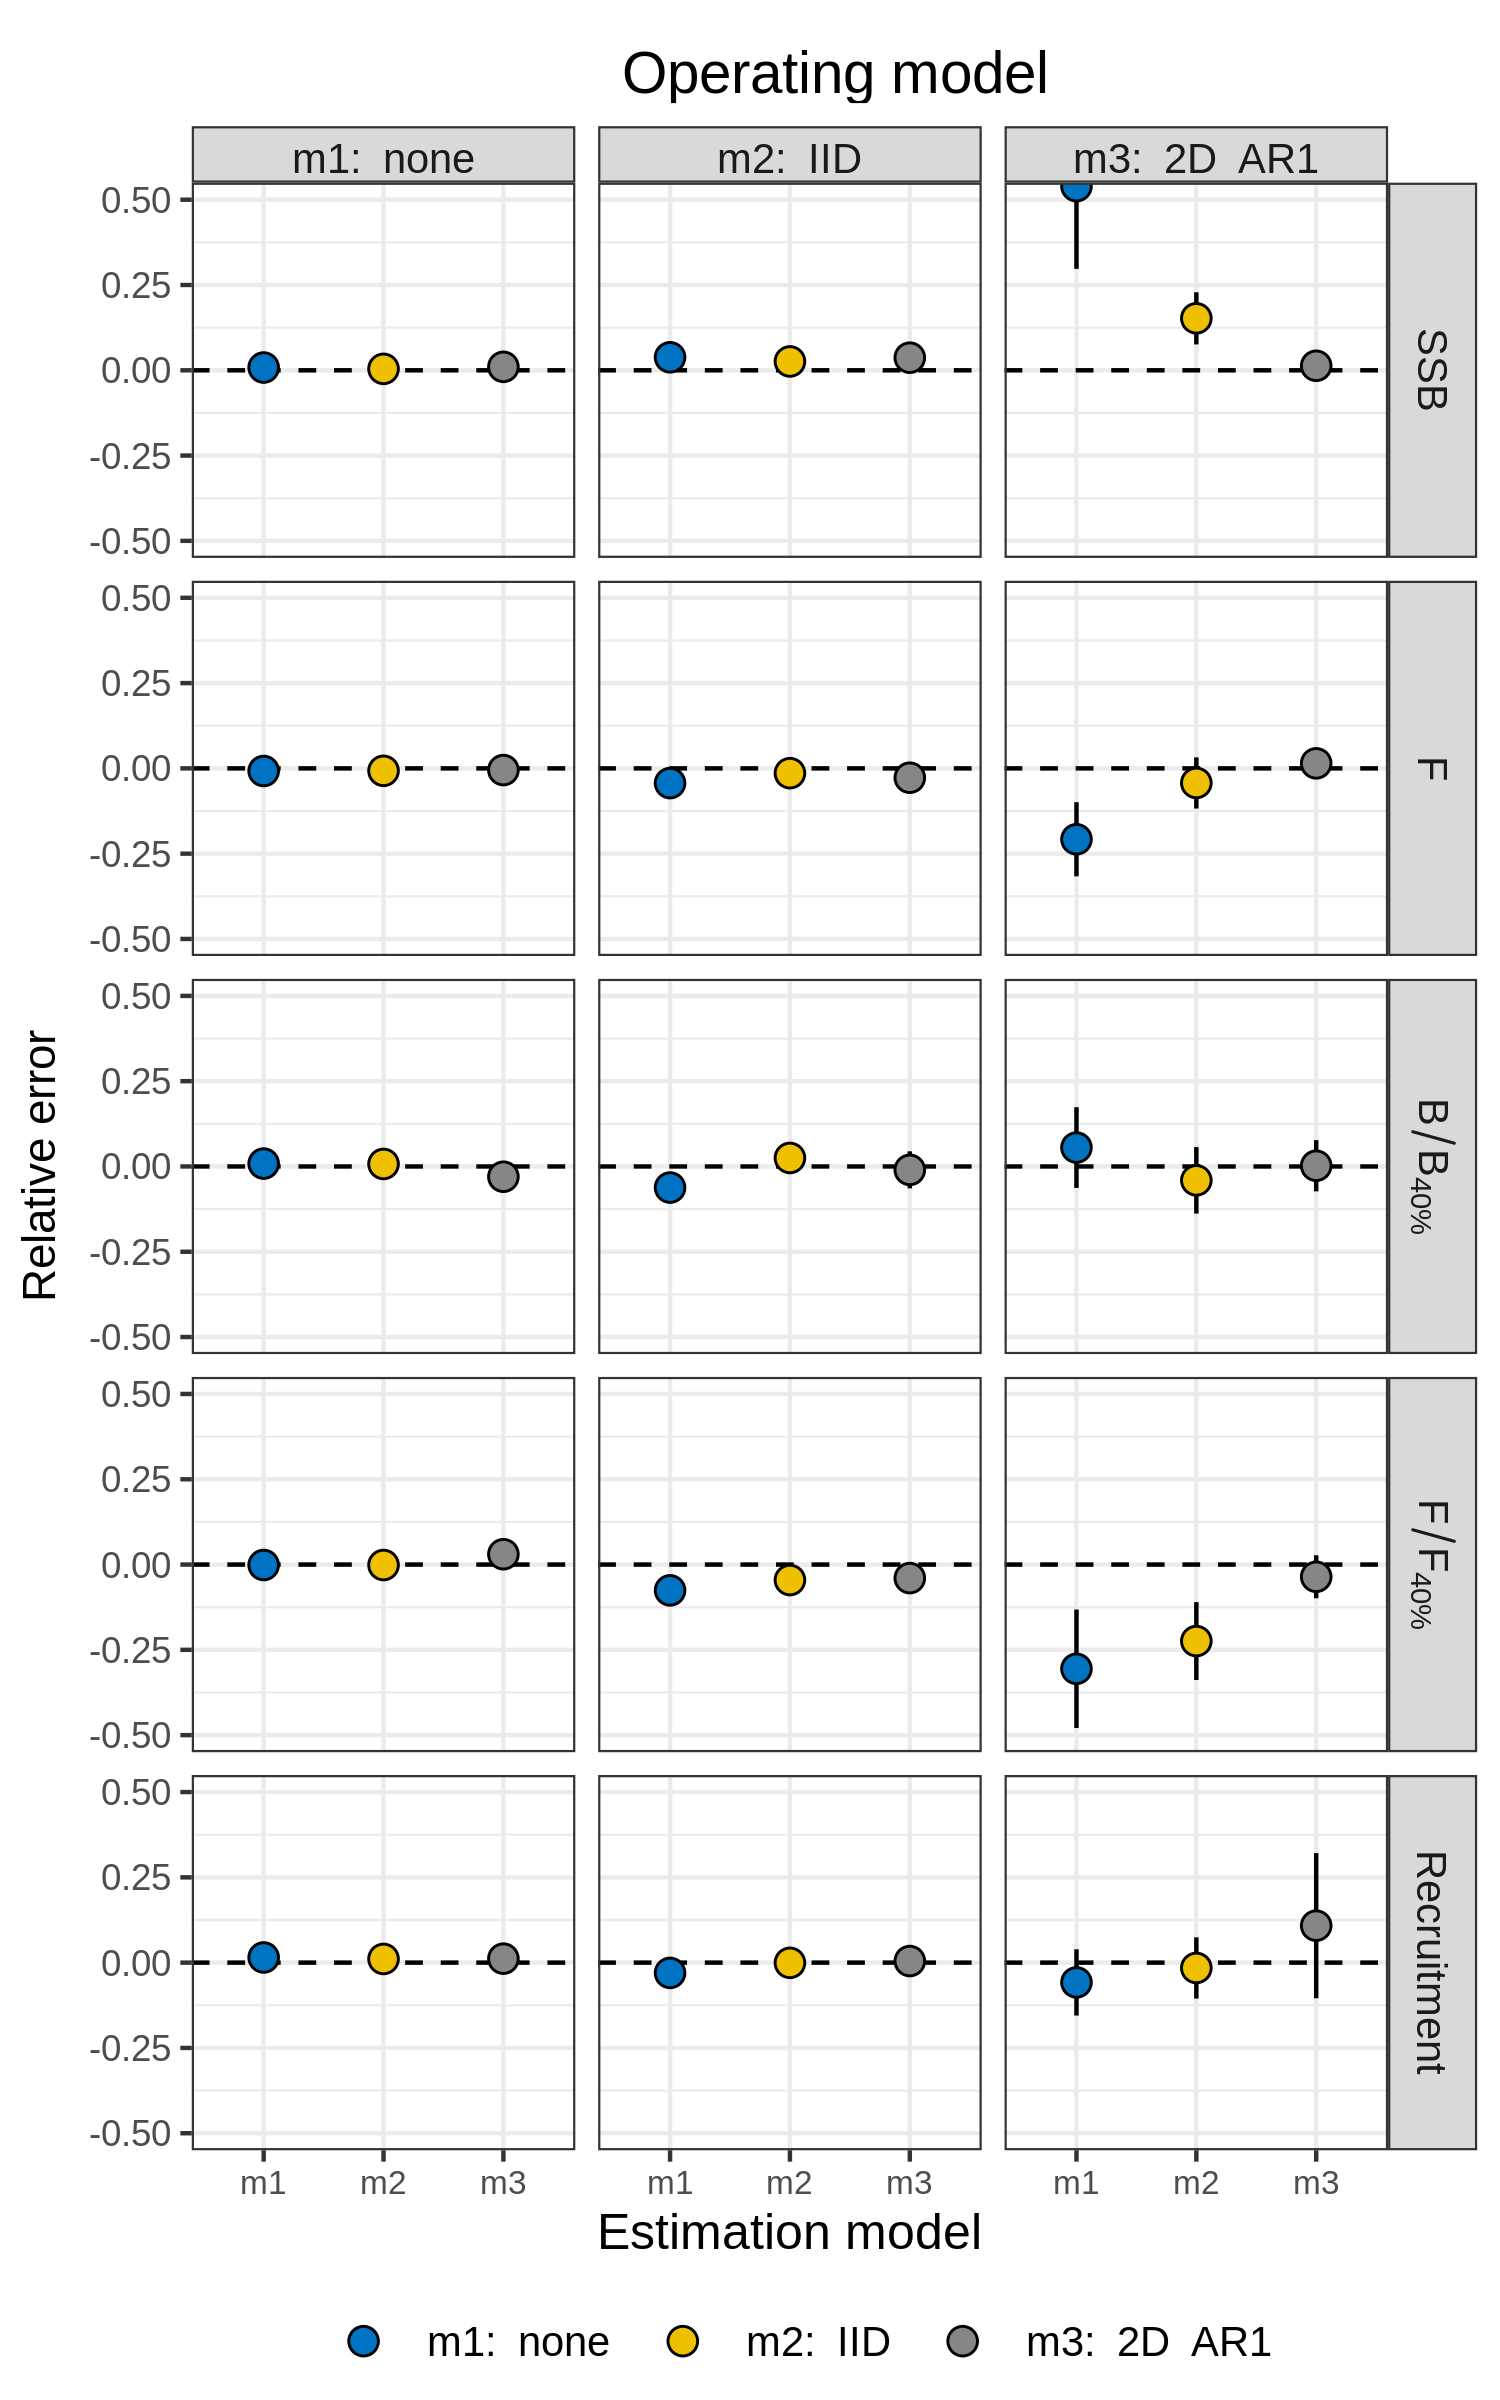
\includegraphics[width=5in]{/home/bstock/Documents/ms/wham-sim/plots/into_paper/0_butterfish_M_medianCI_OEPE} 

}

\caption{Relative error of key quantities estimated for butterfish using three models of natural mortality (\textit{M}) random effects. m1 = no random effects on \textit{M}. m2 = \textit{M} deviations are independent and identically distributed (IID). m3 = \textit{M} deviations are correlated by age and year (2D AR1).}\label{fig:rel-error-butterfish-m}
\end{figure}

\pagebreak

\begin{figure}

{\centering 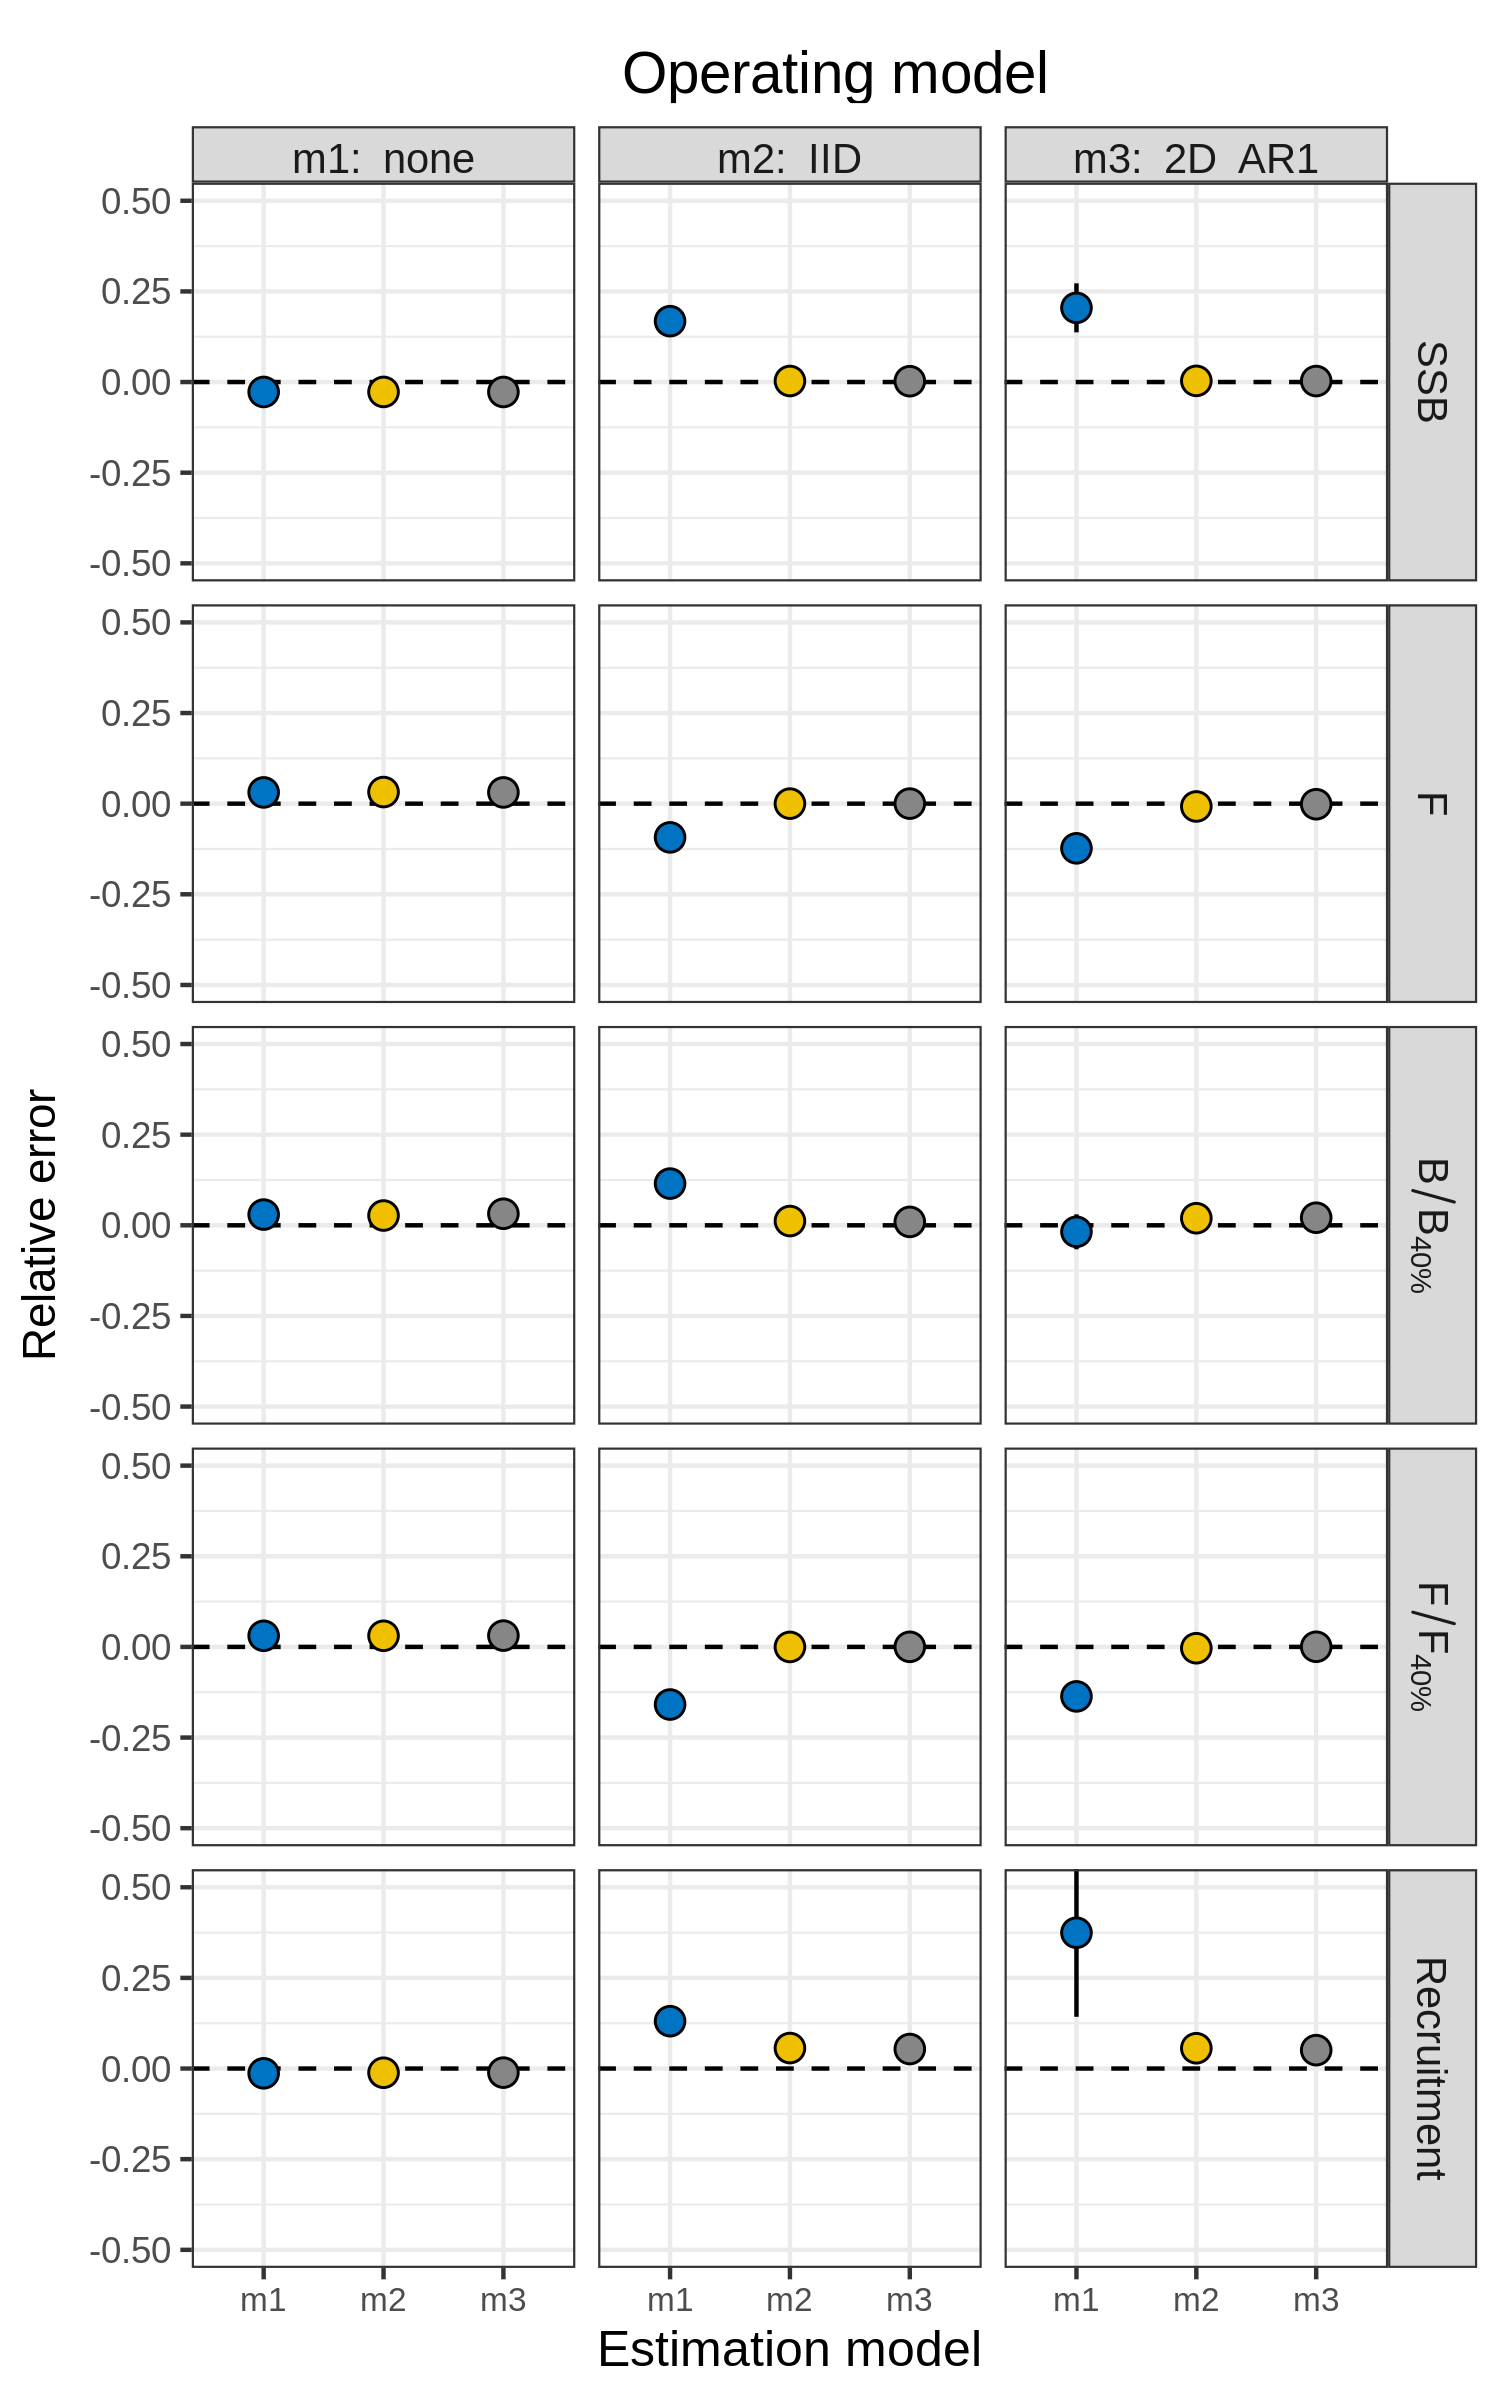
\includegraphics[width=5in]{/home/bstock/Documents/ms/wham-sim/plots/into_paper/0_GBhaddock_sel_medianCI_OEPE} 

}

\caption{Relative error of key quantities estimated for Georges Bank haddock using three models of selectivity random effects. m1 = no random effects (constant logistic selectivity). m2 = selectivity deviations are independent and identically distributed (IID). m3 = selectivity deviations are correlated by parameter and year (2D AR1).}\label{fig:rel-error-GBhaddock-sel}
\end{figure}

\pagebreak

\begin{figure}

{\centering 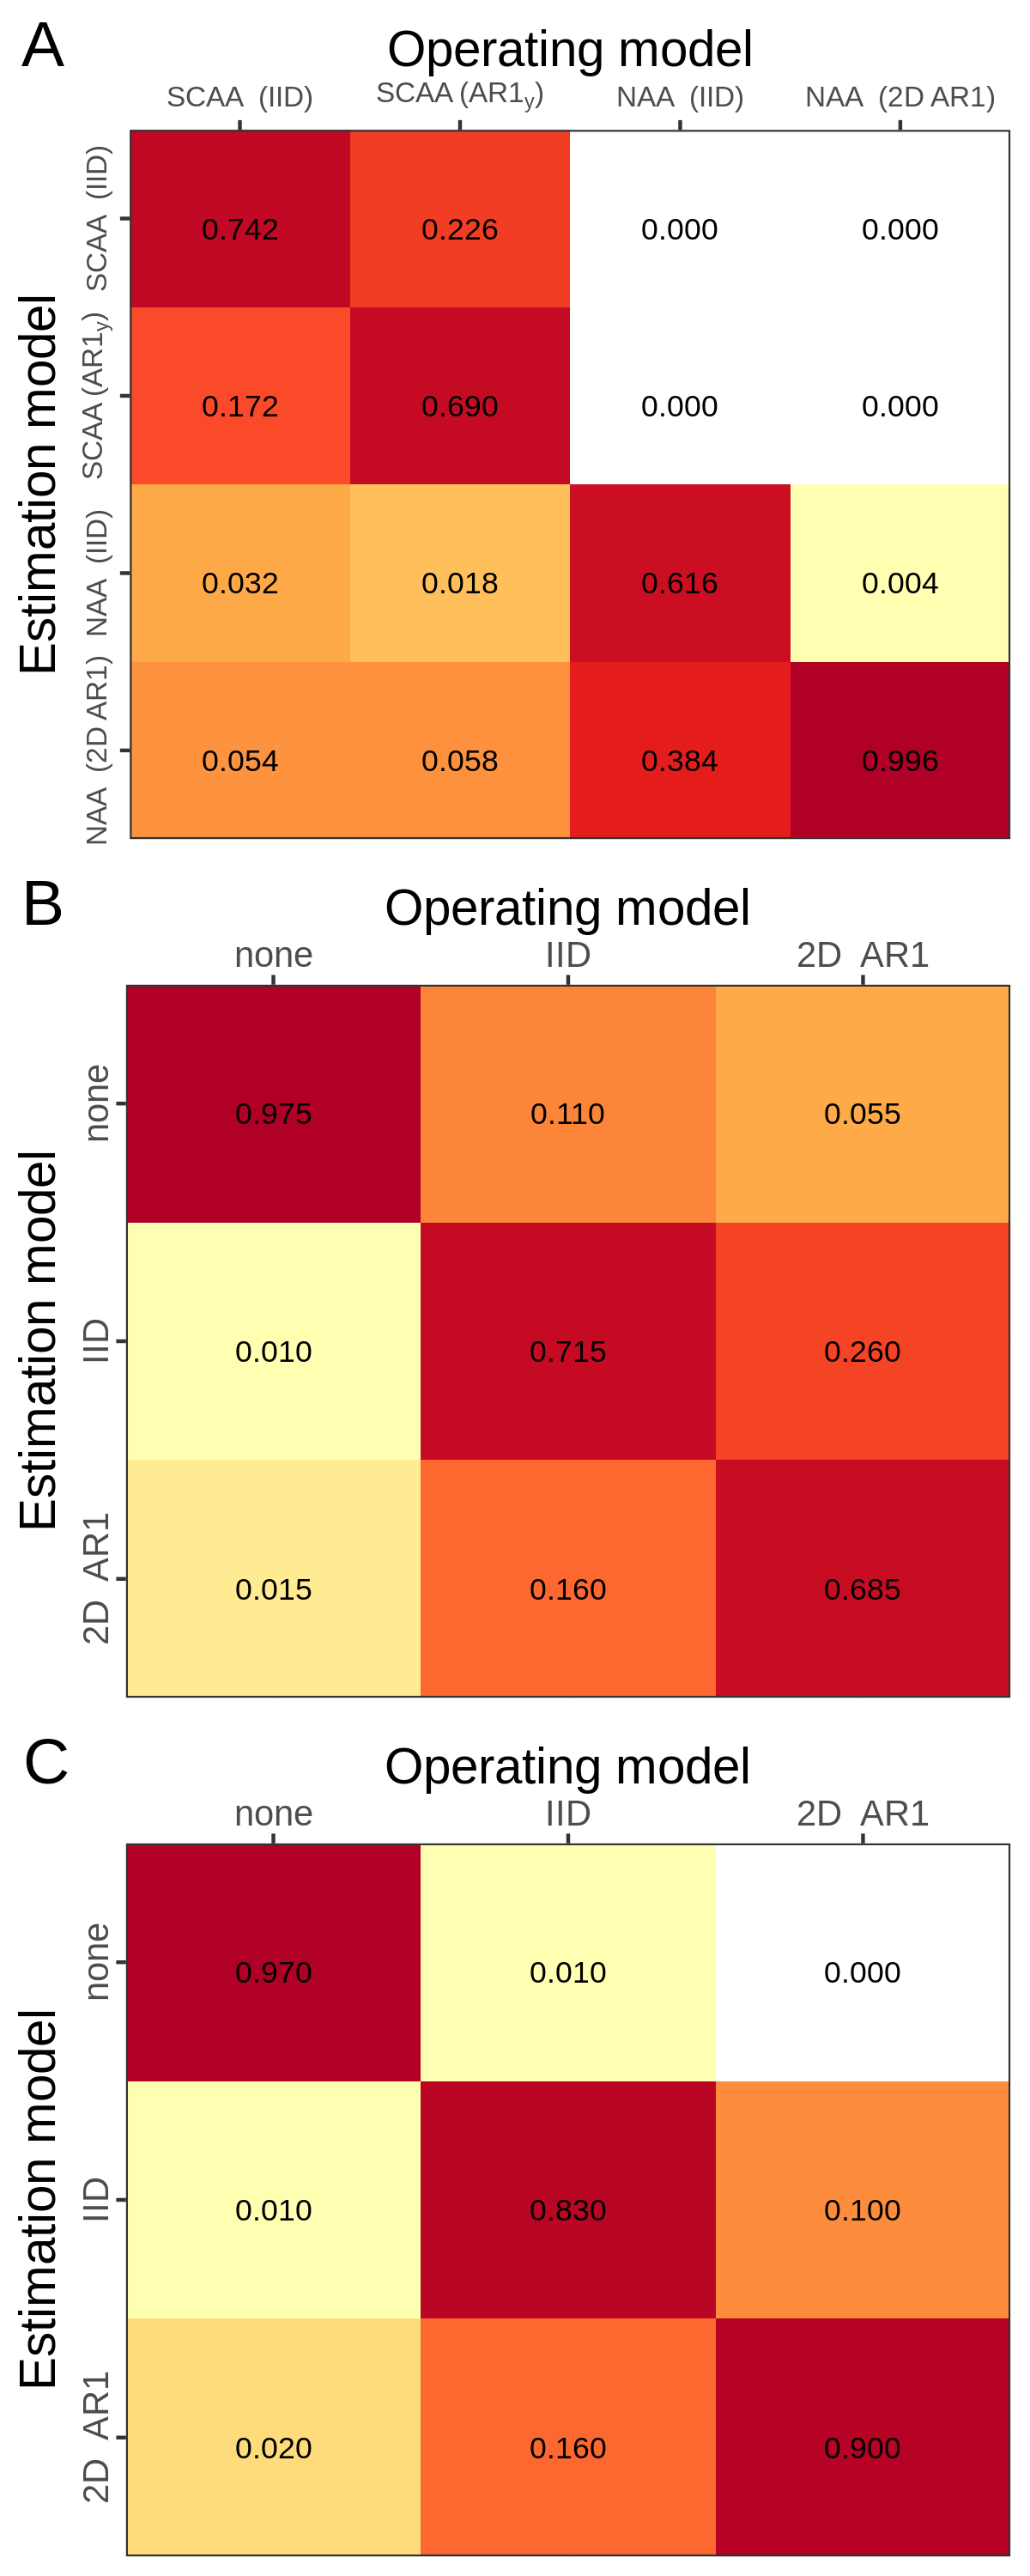
\includegraphics[width=3.5in]{/home/bstock/Documents/ms/wham-sim/plots/into_paper/aic_cross_multipanel} 

}

\caption{Proportion of simulations in which each model had the lowest AIC. A) Numbers-at-age (NAA), aggregated across all five stocks. B) Natural mortality (\textit{M}), aggregated over two stocks (SNEMAYT and NScod). C) Selectivity (GBhaddock). Not all estimation models converged for each simulation, even when the operating model matched.}\label{fig:aic-cross}
\end{figure}

\end{document}
